\subsection{Conics over the Reals}

\begin{tcolorbox}[title=Problem 1, breakable]
    \[P(x,y) = y - x^2, \quad C = \{(x, y) \in \mathbb{R}^2 \mid P(x, y) = 0\}.\]
    Show that for any $(x, y) \in C$, we also have 
    \[(-x, y) \in C.\]
    Thus the curve is symmetric about the y-axis.
\end{tcolorbox}

\begin{proof}
    Let $(x, y) \in C$.
    Then $P(x, y) = y - x^2 = 0$.
    Let $x' = -x$ and note that $(-x)^2 = x^2$.
    Thus
    \[
        P(-x, y) = y - (-x)^2 = y - x^2 = 0.
    \]
    Thus $(-x, y) \in C$.
\end{proof}

\begin{tcolorbox}[title=Problem 2, breakable]
    \[P(x,y) = y - x^2, \quad C = \{(x, y) \in \mathbb{R}^2 \mid P(x, y) = 0\}.\]
    Show that if $(x, y) \in C$, then we have $y \ge 0$.
\end{tcolorbox}

\begin{proof}
    Suppose $(x, y) \in C$.
    Then 
    \[P(x, y) = y - x^2 = 0 \iff y = x^2 \ge 0.\]
    Thus $y \ge 0$.
\end{proof}

\begin{tcolorbox}[title=Problem 3, breakable]
    \[P(x,y) = y - x^2, \quad C = \{(x, y) \in \mathbb{R}^2 \mid P(x, y) = 0\}.\]
    Show that for every $y \ge 0$, there is a point $(x, y) \in C$
    with this $y$-coordinate. Now, for points $(x, y) \in C$, show that if 
    $y$ goes to infinity, then one of the corresponding $x$-coordinates also 
    approaches infinity while the other corresponding $x$ coordinate must approach negative 
    infinity.
\end{tcolorbox}

\begin{proof}
    Let $y \in \mathbb{R}$ such that $y \ge 0$.
    Let $x = \sqrt{y} \in \mathbb{R}$.
    Then
    \[
        y - x^2 = y - (\sqrt{y})^2 = y - y = 0.
    \]
    Thus $(x, y) = (\sqrt{y}, y) \in C$.

    Now suppose $y \to \infty$.
    For points $(x, y) \in C$, we have
    \[
        y - x^2 = 0 \iff x = \pm \sqrt{y}.
    \]
    Since $y \to \infty$, we have $\sqrt{y} \to \infty$ and $-\sqrt{y} \to -\infty$.
    Thus one corresponding $x$-coordinate approaches infinity, while the other
    approaches negative infinity.
\end{proof}

\begin{tcolorbox}[title=Problem 4, breakable]
    Sketch the curve $C = \{(x, y) \in \mathbb{R}^2 \mid P(x, y) = 0\}$.
\end{tcolorbox}

\begin{center}
\begin{tikzpicture}[scale=0.9]
    % Axes
    \draw[->] (-3,0) -- (3,0) node[right] {$x$};
    \draw[->] (0,-1) -- (0,5) node[above] {$y$};

    % Parabola y = x^2
    \draw[domain=-2:2, smooth, thick, blue] plot (\x, {\x*\x});

    % Labels
    \node at (2,4) {$y = x^2$};
\end{tikzpicture}
\end{center}


\begin{tcolorbox}[title=Problem 5, breakable]
    \[C = \left\{(x, y) \in \mathbb{R}^2 \mid \frac{x^2}{4} + \frac{y^2}{9} - 1 = 0 \right\}.\]
    Show that if $(x, y) \in C$, then the three points $(-x, y), (x, -y), (-x, -y)$ are also on $C$.
    Thus the curve $C$ is symmetric about both the $x$- and $y$-axes.
\end{tcolorbox}

\begin{proof}
    Let $(x, y) \in \mathbb{R}^2$.
    Suppose $\frac{x^2}{4} + \frac{y^2}{9} - 1 = 0$.
    Notice that $x^2 = (-x)^2$ and $y = (-y)^2$. Then 
    \[\frac{x^2}{4} + \frac{y^2}{9} - 1 = \frac{(-x)^2}{4} + \frac{y^2}{9} - 1 
                                        = \frac{x^2}{4} + \frac{(-y)^2}{9} - 1 
                                        = \frac{(-x)^2}{4} + \frac{(-y)^2}{9} - 1 = 0.\]
    Thus $(-x, y), (x, -y), (-x, -y) \in C$.
\end{proof}

\begin{tcolorbox}[title=Problem 6, breakable]
    \[C = \left\{(x, y) \in \mathbb{R}^2 \mid \frac{x^2}{4} + \frac{y^2}{9} - 1 = 0 \right\}.\]
    Show that for every $(x, y) \in C$, we have $|x| \le 2$ and $|y| \le 3$.
\end{tcolorbox}

\begin{proof}
    Let $(x, y) \in C$.
    Then 
    \[\frac{x^2}{4} + \frac{y^2}{9} - 1 = 0 \iff 9 x^2 + 4 y^2 - 36 = 0 \iff 9x^2 = -4 y^2 + 36 \iff |x| = \sqrt{\frac{-4}{9} y^2 + 4} \le \sqrt{4} = 2.\]
    Similarly 
    \[9x^2 + 4 y^2 - 36 = 0 \iff |y| = \sqrt{\frac{-9}{4} x^2 + 9} \le \sqrt{9} = 3.\]
\end{proof}

\begin{tcolorbox}[title=Problem 7, breakable]
    Sketch 
    \[C = \left\{(x, y) \in \mathbb{R}^2 \mid \frac{x^2}{4} + \frac{y^2}{9} - 1 = 0 \right\}.\]
\end{tcolorbox}

\begin{center}
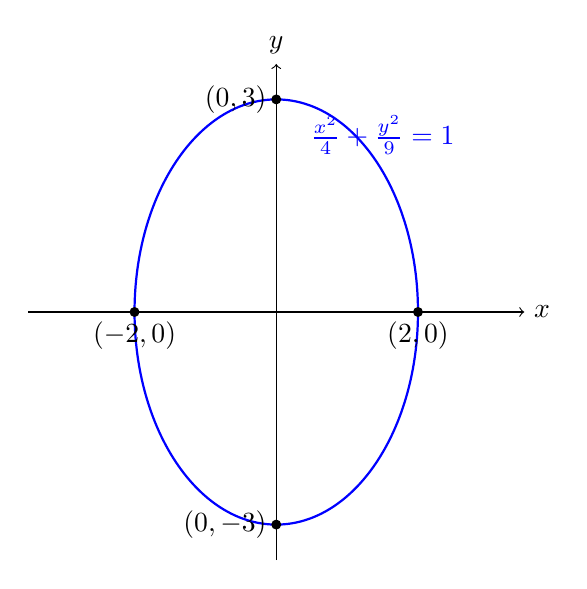
\begin{tikzpicture}[scale=0.9]
    % Axes
    \draw[->] (-3.5,0) -- (3.5,0) node[right] {$x$};
    \draw[->] (0,-3.5) -- (0,3.5) node[above] {$y$};

    % Ellipse: x^2/4 + y^2/9 = 1
    \draw[thick, blue] (0,0) ellipse (2 and 3);

    % Mark key points
    \foreach \x in {-2,2} \fill (\x,0) circle (2pt) node[below] {$(\x,0)$};
    \foreach \y in {-3,3} \fill (0,\y) circle (2pt) node[left] {$(0,\y)$};

    % Label the curve
    \node[blue] at (1.5,2.5) {$\frac{x^2}{4} + \frac{y^2}{9} = 1$};
\end{tikzpicture}
\end{center}

\begin{tcolorbox}[title=Problem 8, breakable]
    \[C = \left\{(x, y) \in \mathbb{R}^2 \mid x^2 - y^2 - 4 = 0\right\}.\]
    Show that if $(x, y) \in C$, then the three points $(-x, y), (x, -y)$, and $(-x, -y)$
    are also on $C$. Thus the curve $C$ is also symmetric about the $x-$ and $y$-axes.
\end{tcolorbox}

\begin{proof}
    Let $(x, y) \in \mathbb{R}^2$.
    Suppose $x^2 - y^2 - 4 = 0$.
    Notice that $x^2 = (-x)^2$ and $y = (-y)^2$. Then 
    \[x^2 - y^2 - 4 = (-x)^2 - y^2 = x^2 - (-y)^2 = (-x)^2 - (-y)^2 = 0.\]
    Thus $(-x, y), (x, -y), (-x, -y) \in C$.
\end{proof}

\begin{tcolorbox}[title=Problem 9, breakable]
    \[C = \left\{(x, y) \in \mathbb{R}^2 \mid x^2 - y^2 - 4 = 0\right\}.\]
    Show that if $(x, y) \in C$, then we have $|x| \ge 2$.
\end{tcolorbox}

\begin{proof}
    Let $(x, y) \in \mathbb{R}^2$.
    Suppose $x^2 - y^2 - 4 = 0$.
    Then 
    \[x^2 - y^2 - 4 = 0 \iff x^2 = y^2 + 4 \iff |x| = \sqrt{y^2 + 4} \ge \sqrt{4} = 2.\]
\end{proof}

\begin{tcolorbox}[title=Problem 10, breakable]
    \[C = \left\{(x, y) \in \mathbb{R}^2 \mid x^2 - y^2 - 4 = 0\right\}.\]
    Show that the curve $C$ is unbounded in the positive 
        and negative $x$-directions and also unbounded in the 
        positive and negative $y$-directions.
\end{tcolorbox}

\begin{proof}
    First notice
    \[
        x^2 - y^2 - 4 = 0 
        \iff x^2 = y^2 + 4 
        \iff x = \pm \sqrt{y^2 + 4}
        \iff y = \pm \sqrt{x^2 - 4}.
    \]
    As $y \to \infty$, we have $x = \pm \sqrt{y^2 + 4} \to \infty$ and $-\infty$.
    Similarly, as $x \to \infty$, we have $y = \pm \sqrt{x^2 - 4} \to \infty$ and $-\infty$.
\end{proof}


\begin{tcolorbox}[title=Problem 11, breakable]
    Sketch 
    \[C = \left\{(x, y) \in \mathbb{R}^2 \mid x^2 - y^2 - 4 = 0\right\}.\]
\end{tcolorbox}

\begin{center}
\begin{tikzpicture}[scale=0.8]
    % Axes
    \draw[->] (-6,0) -- (6,0) node[right] {$x$};
    \draw[->] (0,-5) -- (0,5) node[above] {$y$};

    % Hyperbola x^2 - y^2 = 4
    \draw[domain=-5:-2, smooth, thick, blue] 
        plot (\x, {sqrt(\x*\x - 4)});
    \draw[domain=-5:-2, smooth, thick, blue] 
        plot (\x, {-sqrt(\x*\x - 4)});
    \draw[domain=2:5, smooth, thick, blue] 
        plot (\x, {sqrt(\x*\x - 4)});
    \draw[domain=2:5, smooth, thick, blue] 
        plot (\x, {-sqrt(\x*\x - 4)});

    % Asymptotes y = ±x
    \draw[dashed] (-5,-5) -- (5,5);
    \draw[dashed] (-5,5) -- (5,-5);

    % Label
    \node[blue] at (3.5,2.5) {$x^2 - y^2 = 4$};
\end{tikzpicture}
\end{center}

\begin{tcolorbox}[title=Problem 12, breakable]
    Sketch the graph of each of the following conics in 
        $\mathbb{R}^2$.
    Identify which are parabolas, ellipses, or Hyperbola.
    \begin{enumerate}
        \item $V(x^2 - 8y)$.
        \item $V(x^2 + 2x - y^2 - 3y - 1)$.
        \item $V(4x^2 + y^2)$.
        \item $V(3x^2 + 3y^2 - 75)$.
        \item $V(x^2 - 9y^2)$.
        \item $V(4x^2 + y^2 - 8)$.
        \item $V(x^2 + 9y^2 - 36)$.
        \item $V(x^2 - 4 y^2 - 16)$.
        \item $V(y^2 - x^2 - 9)$.
    \end{enumerate}
\end{tcolorbox}

\textbf{Solution (1):}
Parabola.
\begin{figure}[h!]
    \centering
    \includegraphics[width=0.3\textwidth]{images/chapter1/1.png}
\end{figure}

\textbf{Solution (2):}
Hyperbola.
\begin{figure}[h!]
    \centering
    \includegraphics[width=0.3\textwidth]{images/chapter1/2.png}
\end{figure}

\textbf{Solution (3):}
Point.

\textbf{Solution (4):}
Ellipse.
\begin{figure}[h!]
    \centering
    \includegraphics[width=0.3\textwidth]{images/chapter1/4.png}
\end{figure}

\textbf{Solution (5):}
Two lines.
\begin{figure}[h!]
    \centering
    \includegraphics[width=0.3\textwidth]{images/chapter1/5.png}
\end{figure}

\textbf{Solution (6):}
Ellipse.
\begin{figure}[h!]
    \centering
    \includegraphics[width=0.3\textwidth]{images/chapter1/6.png}
\end{figure}

\textbf{Solution (7):}
Ellipse.
\begin{figure}[h!]
    \centering
    \includegraphics[width=0.3\textwidth]{images/chapter1/7.png}
\end{figure}

\textbf{Solution (8):}
Hyperbola.
\begin{figure}[h!]
    \centering
    \includegraphics[width=0.3\textwidth]{images/chapter1/8.png}
\end{figure}

\textbf{Solution (9):}
Hyperbola.
\begin{figure}[h!]
    \centering
    \includegraphics[width=0.3\textwidth]{images/chapter1/9.png}
\end{figure}

\begin{tcolorbox}[title=Problem 13, breakable]
    Express the polynomial $P(x, y) = ax^2 + bxy + cy^2 + dx + ey + h$ in the form
    \[P(x, y) = Ax^2 + Bx + C,\]
    where $A, B$, and $C$ are polynomials in $y$. What are $A, B$, and $C$?
\end{tcolorbox}

\begin{proof}
    Let $A = a, B = by + d$, and $C = cy^2 + ey + h$.
    Notice 
    \[
    ax^2 + bxy + cy^2 + dx + ey + h
    = a x^2 + bxy + dx + cy^2 + ey + h
    = a x^2 + (by + d)x + (cy^2 + ey + h)
    = Ax^2 + Bx + C.
    \]
\end{proof}

\begin{tcolorbox}[title=Problem 14, breakable]
    Treating $P(x, y) = ax^2 + bxy + cy^2 + dx + cy + h$ as a polynomial
    in the variable $x$, show that the discriminant is 
    \[\triangle_x (y) = (b^2 - 4ac)y^2 + (2bd - 4ae)y + (d^2 - 4ah).\]
\end{tcolorbox}

\begin{proof}
    From Problem 13 we have $A = a, B = by + d$, and $C = cy^2 + ey + h$.
    Then 
    \[
    \triangle_x (y) = B^2 - 4AC
    = (by + d)^2 - 4a(cy^2 + ey + h)
    = (b^2 - 4ac)y^2 + (2bd - 4ae)y + (d^2 - 4ah).
    \]
\end{proof}

\begin{tcolorbox}[title=Problem 15, breakable]
    \begin{enumerate}
        \item Suppose $\triangle_x (y_0) < 0$. Explain why there is no point on $V(p)$ whose $y$-coordinate is $y_0$.
        \item Suppose $\triangle_x (y_0) = 0$. Explain why there is exactly one point on $V(P)$ whose $y$-coordinate is $y_0$.
        \item Suppose $\triangle_x (y_0) > 0$. Explain why there are exactly two points on $V(P)$ whose $y$-coordinate is $y_0$.
    \end{enumerate}
\end{tcolorbox}

\textbf{Solution (a):} In $\mathbb{R}$, the square root is undefined for values $< 0$.

\textbf{Solution (b):} If $\triangle_x (y_0) = 0$, then $+\sqrt{B^2 - 4AC} = -\sqrt{B^2 - 4AC}$,  
so there is exactly one point on $V(P)$ whose $y$-coordinate is $y_0$.

\textbf{Solution (c):} If $\triangle_x (y_0) > 0$, then $+\sqrt{B^2 - 4AC} \ne -\sqrt{B^2 - 4AC}$,  
so there are exactly two points on $V(P)$ whose $y$-coordinate is $y_0$.

\begin{tcolorbox}[title=Problem 16, breakable]
    Suppose $b^2 - 4ac = 0$. Suppose further that $2bd - 4 ae > 0$.
    \begin{enumerate}
        \item Show that $\triangle_x (y) \ge 0$ if and only if $y \ge \frac{4 ah - d^2}{2bd - 4ae}$.
        \item Conclude that if $b^2 - 4ac = 0$ and $2bd - 4ae > 0$, then $V(P)$ is a parabola.
    \end{enumerate}
\end{tcolorbox}

\begin{proof}
    Suppose $\triangle_x (y) \ge 0$.
    Then 
    \begin{align*}
        \triangle_x (y) &= (b^2 - 4ac)y^2 + (2bd - 4ae)y + (d^2 - 4ah) \\
                        &= 0 y^2 + (2bd - 4 ae)y + (d^2 - 4ah).
    \end{align*}
    Therefore,
    \[
        (2bd - 4ae)y + (d^2 - 4ah) \ge 0.
    \]
    Since $2bd - 4ae > 0$, we have
    \[
        y \ge \frac{4ah - d^2}{2bd - 4ae}.
    \]
    Conversely, suppose $y \ge \frac{4ah - d^2}{2bd - 4ae}$.
    Then 
    \begin{align*}
        \triangle_x (y) &= (2bd - 4ae)y + (d^2 - 4ah) \\
                        &\ge (2bd - 4ae)\left(\frac{4ah - d^2}{2bd - 4ae}\right) + (d^2 - 4ah) \\
                        &= 0.
    \end{align*}
\end{proof}

\begin{proof}
    Suppose $b^2 - 4ac = 0$ and $2bd - 4ae > 0$.
    Then $\triangle_x (y) = (2bd - 4ae)y + (d^2 - 4ah)$.
    Now, $x = \frac{-B \pm \sqrt{B^2 - 4AC}}{2A}$.
    It is clear that $x$ is symmetrical, and since $y \ge \frac{4ah - d^2}{2bd - 4ae}$,
    $V(P)$ is a parabola.
\end{proof}


\begin{tcolorbox}[title=Problem 17, breakable]
    Suppose $b^2 - 4ac < 0$.
    \begin{enumerate}
        \item Show that one of the following occurs:
        \begin{enumerate}
            \item $\{y \mid \triangle_x (y) \ge 0\} = \emptyset$,
            \item $\{y \mid \triangle_x (y) \ge 0\} = \{y_o\}$,
            \item there exist real numbers $\alpha$ and $\beta$, $\alpha < \beta$, such that 
            \[\{y \mid \triangle_x (y) \ge 0\} = \{y \mid \alpha \le y \le \beta\}.\]
        \end{enumerate}
        \item Conclude that $V(P)$ is either emptyset, a point, or an ellipse.
    \end{enumerate}
\end{tcolorbox}

\begin{proof}
    Since $b^2 - 4ac < 0$, the graph of
    $\triangle_x(y)$ is a downward opening parabola in $y$.
    There are three cases, depending on the number of real zeros of $\triangle_x(y)$.
    \begin{enumerate}
        \item If $\triangle_x(y) < 0$ for all $y$, then
        \[
            \{y \mid \triangle_x(y) \ge 0\} = \emptyset.
        \]
        \item If $\triangle_x(y)$ has exactly one real zero $y_0$, then
        \[
            \{y \mid \triangle_x(y) \ge 0\} = \{y_0\}.
        \]
        \item If $\triangle_x(y)$ has two distinct real zeros $\alpha < \beta$, then
        \[
            \{y \mid \triangle_x(y) \ge 0\} = \{y \mid \alpha \le y \le \beta\}.
        \]
    \end{enumerate}
\end{proof}

\begin{proof}
    From part 1 the set of $y$ values is either empty, a single point, or a bounded interval, it follows that
        $V(P)$ is either empty, a point, or an ellipse.
\end{proof}


\begin{tcolorbox}[title=Problem 18, breakable]
    Suppose $b^2 - 4ac > 0$.
    \begin{enumerate}
        \item Show that one of the following occurs:
        \begin{enumerate}
            \item $\{y \mid \triangle_x (y) \ge 0\} = \mathbb{R}$ and $\triangle_x (y) \ne 0$,
            \item $\{y \mid \triangle_x (y) = 0\} = \{y_0\}$ and $\{y \mid \triangle_x (y) > 0\} = \{y \mid y \ne y_0\}$,
            \item there exist real numbers $\alpha$ and $\beta$, $\alpha < \beta$, such that 
            \[\{y \mid \triangle_x (y) \ge 0\} = \{y \mid y \le \alpha\} \cup \{y \mid y \ge \beta\}.\]
        \end{enumerate}
        \item If $\{y \mid \triangle_x (y)\} = \mathbb{R}$, show that $V(P)$ is a hyperbola opening left and right.
        \item If $\{y \mid \triangle_x (y) = 0\} = \{y_0\}$, show that $V(P)$ is two lines intersecting in a point.
        \item If there are two real numbers $\alpha$ and $\beta$, $\alpha < \beta$, such that 
        \[\{y \mid \triangle_x (y) \ge 0\} = \{y \mid y \le \alpha\} \cup \{y \mid y \ge \beta\},\]
        show that $V(P)$ is a hyperbola opening up and down.
    \end{enumerate}
\end{tcolorbox}

\begin{proof}
    Since $b^2 - 4ac > 0$, the graph of
    $\triangle_x(y)$ is an upward opening parabola in $y$.
    There are three cases, depending on the number of real zeros of $\triangle_x(y)$.
    \begin{enumerate}
        \item If $\triangle_x(y) > 0$ for all $y$, then
        \[
            \{y \mid \triangle_x(y) \ge 0\} = \mathbb{R}.
        \]
        \item If $\triangle_x(y)$ has exactly one real zero $y_0$, then
        \[
            \{y \mid \triangle_x (y) = 0\} = \{y_0\}
            \quad \text{and} \quad
            \{y \mid \triangle_x (y) > 0\} = \{y \mid y \ne y_0\}.
        \]
        \item If $\triangle_x(y)$ has two distinct real zeros $\alpha < \beta$, then
        \[
            \{y \mid \triangle_x (y) \ge 0\}
            = \{y \mid y \le \alpha\} \cup \{y \mid y \ge \beta\}.
        \]
    \end{enumerate}
\end{proof}

\begin{proof}
    Since $b^2 - 4ac > 0$, the graph of
    $\triangle_x(y)$ is an upward opening parabola in $y$.
    There are three cases, depending on the number of real zeros of $\triangle_x(y)$.
    \begin{enumerate}
        \item If $\triangle_x(y) > 0$ for all $y$, then
        \[
            \{y \mid \triangle_x(y) \ge 0\} = \mathbb{R}.
        \]
        \item If $\triangle_x(y)$ has exactly one real zero $y_0$, then
        \[
            \{y \mid \triangle_x (y) = 0\} = \{y_0\}
            \quad \text{and} \quad
            \{y \mid \triangle_x (y) > 0\} = \{y \mid y \ne y_0\}.
        \]
        \item If $\triangle_x(y)$ has two distinct real zeros $\alpha < \beta$, then
        \[
            \{y \mid \triangle_x (y) \ge 0\}
            = \{y \mid y \le \alpha\} \cup \{y \mid y \ge \beta\}.
        \]
    \end{enumerate}
\end{proof}

\begin{proof}
    Suppose $\{y \mid \triangle_x (y) \ge 0\} = \mathbb{R}$.
    Then for every $y$ there exist two real solutions for $x$, and $x$ is unbounded
    to the left and right. Since the equation is quadratic in $x$, the curve is
    symmetric in $x$.
    Thus $V(P)$ is a hyperbola opening left and right.
\end{proof}

\begin{proof}
    Suppose $\{y \mid \triangle_x (y) = 0\} = \{y_0\}$.
    Then for $y = y_0$ the equation has exactly one real solution for $x$, and for
    $y \ne y_0$ it has two real solutions. Since the equation is quadratic in $x$,
    $V(P)$ consists of two lines intersecting at a point.
\end{proof}

\begin{proof}
    Suppose there exist real numbers $\alpha$ and $\beta$, $\alpha < \beta$, such that
    \[
        \{y \mid \triangle_x (y) \ge 0\}
        = \{y \mid y \le \alpha\} \cup \{y \mid y \ge \beta\}.
    \]
    For $y \le \alpha$ or $y \ge \beta$, the equation has two real solutions in $x$.
    If $\alpha < y < \beta$ it has no real solutions. Thus $x$ is bounded for each
    $y$, but $y$ is unbounded above and below.
    Since the equation is quadratic in $x$, the curve is symmetric in $x$.
    Therefore $V(P)$ is a hyperbola opening up and down.
\end{proof}

\begin{tcolorbox}[title=Problem 19, breakable]
    Show that the discriminant of $A'y^2 + B'y + C' = 0$ is 
    \[\triangle_y (x) = (b^2 - 4ac)x^2 + (2be - 4cd)x + (e^2 - 4ch).\]
\end{tcolorbox}

\begin{proof}
    Here $A' = c$, $B' = bx + e$, and $C' = ax^2 + dx + h$. Then
    \[
        \triangle_y(x) = (B')^2 - 4 A' C'
        = (bx + e)^2 - 4 c (ax^2 + dx + h)
        = (b^2 - 4ac)x^2 + (2be - 4cd)x + (e^2 - 4ch).
    \]
\end{proof}

\subsection{Changes of Coordinates}

\begin{tcolorbox}[title=Problem 1, breakable]
    Show that the origin in the $xy$-coordinate system 
    agrees with the origin in the $uv$-system if and only if 
    $e = f = 0$. Thus the constants $e$ and $f$ describe 
    translations of the origin.
\end{tcolorbox}

\begin{proof}
    Suppose the $xy$-coordinate system agrees with the origin 
        of the $uv$-system.
    Then 
    \[u = 0 = a(0) + b(0) + e = e,\] 
    and 
    \[v = 0 = c(0) + d(0) + f = f.\]
    Thus $f = e = 0$.

    Conversely, suppose $e = f = 0$.
    Then 
    \[u = ax + by + e = ax + by + 0 = a(0) + b(0) = 0,\]
    and 
    \[v = cx + dy + f = cx + dy + 0 = c(0) + d(0) = 0.\]
    Thus the origin of the $xy$-coordinate system agrees with the 
        origin of the $uv$-system.
\end{proof}


\begin{tcolorbox}[title=Problem 2, breakable]
    Show that if $u = ax + by + e$ and $v = cx + dy + f$ 
        is a change of coordinates, then the inverse change of 
        coordinates is 
    \[x = \left( \frac{1}{ad - bc} \right) (du - bv) - \left( \frac{1}{ad - bc} \right) (de - bf).\]
    \[y = \left( \frac{1}{ad - bc} \right) (-cu + av ) - \left( \frac{1}{ad - bc} \right) (-ce + af).\]
\end{tcolorbox}

\begin{proof}
    We need to solve the two equations $u = ax + by + e$ and $v = cx + dy + f$ in two unknowns $x$ and $y$.
    Translating this to linear algebra, we have 
    \[
        \begin{bmatrix}
            a & b \\
            c & d
        \end{bmatrix}
        \begin{bmatrix}
            x \\ 
            y
        \end{bmatrix} = 
        \begin{bmatrix}
            u - e \\
            v - f
        \end{bmatrix}.
    \]
    Using Cramer's rule we see
    \[
        x = \frac{
            \begin{vmatrix} u - e & b \\ v - f & d \end{vmatrix}
        }{
            \begin{vmatrix} a & b \\ c & d \end{vmatrix}}
        = \frac{d(u-e) - b(v-f)}{ad - bc},
    \]
    \[
        y = \frac{
            \begin{vmatrix} a & u - e \\ c & v - f \end{vmatrix}
        }{
            \begin{vmatrix} a & b \\ c & d \end{vmatrix}}
        = \frac{-c(u-e) + a(v-f)}{ad - bc}.
    \]
    Therefore
    \[
        x = \frac{du - bv - de + bf}{ad - bc}, \quad
        y = \frac{-cu + av + ce - af}{ad - bc}.
    \]
\end{proof}


\begin{tcolorbox}[title=Problem 3, breakable]
    Show that if 
    \[u = ax + by + e\]
    \[v = cx + dy + f,\]
    and 
    \[s = Au + Bv + E\]
    \[t = Cu + Dv + F\]
    are two real affine changes of coordinates from the $xy$-plane
    to the $uv$-plane and from the $uv$-plane to the $st$-plane, respectively,
    then the composition from the $xy$-plane to the $st$-plane is a real 
    affine change of coordinates.
\end{tcolorbox}

\begin{proof}
    Suppose
    \[u = ax + by + e\]
    \[v = cx + dy + f,\]
    and 
    \[s = Au + Bv + E\]
    \[t = Cu + Dv + F\]
    are two real affine changes of coordinates from the $xy$-plane
    to the $uv$-plane and from the $uv$-plane to the $st$-plane respectively.
    Substituting $u, v$ into $s, t$ we see 
    \[s = A(ax + by + e) + B(cx + dy + f) + E = (Aa + Bc)x + (Ab + Bd)y + (Ae + Bf + E),\]
    and
    \[t = C(ax + by + e) + D(cx + dy + f) + F = (Ca + Dc)x + (Cb + Dd)y + (Ce + Df + F).\]
    Finally,
    \[\det\left(\begin{bmatrix}
        Aa + Bc & Ab + Bd \\
        Ca + Dc & Cb + Dd
    \end{bmatrix}\right)
    = (Aa + Bc)(Cb + Dd) - (Ab + Bd)(Ca + Dc)
    = (ad - bc)(AD - BC) \ne 0.\]
\end{proof}


\begin{tcolorbox}[title=Problem 4, breakable]
    For each affine pair of ellipses, find a real affine change 
        of coordinates that maps the ellipse in the $xy$-plane 
        to the ellipse in the $uv$-plane.
    \begin{enumerate}
        \item $V(x^2 + y^2 - 1), V(16 u^2 + 9v^2 - 1)$.
        \item $V((x - 1)^2 + y^2 - 1), V(16 u^2 + 9(v + 2)^2 - 1)$.
        \item $V(4 x^2 + y^2 - 6y + 8), V(u^2 - 4u + v^2 - 2v + 4)$.
        \item $V(13 x^2 - 10 xy + 13 y^2 - 1), V(4 u^2 + 9 v^2 - 1)$.
    \end{enumerate}
\end{tcolorbox}

\textbf{Solution (1):}
Let $x = 4u$ and $y = 3v$.
Then 
\[x^2 + y^2 - 1 = (4u)^2 + (3v)^2 - 1 = 16 u^2 + 9 v^2 - 1 = 0.\]
\textbf{Solution (2):}
Let $x = 4u + 1$ and $y = 3v + 6$.
Then 
\[(x - 1)^2 + y^2 - 1 = (4u + 1 - 1)^2 + (3v + 6)^2 = 16 u^2 + 9(v + 2)^2 = 0.\]
\textbf{Solution (3):}
Let $x = \frac{u}{2} - 1$ and $y = v + 2$.
Then 
\[4 x^2 + y^2 - 6y + 8 = 4\left(\frac{u}{2} - 1\right)^2 + (v + 2)^2 - 6(v + 2) + 8 =\] 
\[4\left(\frac{u^2}{4} - 2 \frac{u}{2} + 1\right) + v^2 + 4v + 4 - 6v - 12 + 8 = u^2 - 4u + 4 + v^2 - 2v = u^2 - 4u + v^2 - 2v + 4.\]
\textbf{Solution (4):} 
Let $x = \frac{u+v}{2}$ and $y = \frac{u-v}{2}$.
Then 
\[
13x^2 - 10xy + 13y^2 - 1 = 13\left(\frac{u+v}{2}\right)^2 - 10\left(\frac{u+v}{2}\cdot \frac{u-v}{2}\right) + 13\left(\frac{u-v}{2}\right)^2 - 1
\] 
\[
= 13\frac{(u+v)^2}{4} - 10\frac{u^2 - v^2}{4} + 13\frac{(u-v)^2}{4} - 1
\] 
\[
= \frac{13}{4}(u^2 + 2uv + v^2) - \frac{10}{4}(u^2 - v^2) + \frac{13}{4}(u^2 - 2uv + v^2) - 1
\] 
\[
= \frac{13+13-10}{4} u^2 + \frac{13+13+10}{4} v^2 + \frac{26-26}{4} uv - 1
\] 
\[
= 4 u^2 + 9 v^2 - 1.
\]


\begin{tcolorbox}[title=Problem 5, breakable]
    For each pair of hyperbolas, find a real affine change 
    of coordinates that maps the hyperbola in the $xy$-plane to the 
    hyperbola in the $uv$-plane.
    \begin{enumerate}
        \item $V(xy - 1), V(u^2 - v^2 - 1)$.
        \item $V(x^2 - y^2 - 1), V(16 u^2 - 9v^2 - 1)$.
        \item $V((x - 1)^2 - y^2 - 1), V(16 u^2 - 9(v + 2)^2 - 1)$.
        \item $V(x^2 - y^2 - 1), V(v^2 - u^2 - 1)$.
        \item $V(8xy - 1), V(2u^2 - 2v^2 - 1)$.
    \end{enumerate}
\end{tcolorbox}

\textbf{Solution (1):}
Let $x = u - v$ and $y = u + v$.
Then 
\[xy - 1 = (u - v)(u + v) - 1 = u^2 - v^2 - 1.\]
\textbf{Solution (2):}
Let $x = 4u$ and $y = 3v$.
Then 
\[x^2 - y^2 - 1 = (4u)^2 - (3v)^2 - 1 = 16 u^2 - 9v^2 - 1.\]
\textbf{Solution (3):}
Let $x = 4u + 1$ and $y = 3v + 6$.
Then 
\[(x - 1)^2 - y^2 - 1 = (4u + 1 - 1)^2 - (3v + 6)^2 = 16 u^2 - 9(v + 2)^2 - 1.\]
\textbf{Solution (4):}
Let $x = v$ and $y = u$.
Then 
\[x^2 - y^2 - 1 = v^2 - u^2 - 1.\]
\textbf{Solution (5):}
Let $x = (u + v)/4$ and $y = (u - v)/2$.
Then 
\[8xy - 1 = 8((u + v)/4)((u - v)/2) - 1 = (u + v)(u - v) - 1 = u^2 - v^2 - 1.\]


\begin{tcolorbox}[title=Problem 6, breakable]
    For each pair of parabolas, find a real affine change 
    of coordinates that maps the parabola in the $xy$-plane 
    to the parabola in the $uv$-plane.
    \begin{enumerate}
        \item $V(x^2 - y), V(9v^2 - 4u)$.
        \item $V((x - 1)^2 - y), V(u^2 - 9(v + 2))$.
        \item $V(x^2 - y), V(u^2 + 2uv + v^2 - u + v - 2)$.
        \item $V(x^2 - 4x + y + 4), V(4u^2 - (v + 1))$.
        \item $V(4x^2 + 4xy + y^2 - y + 1), V(4 u^2 + v)$.
    \end{enumerate}
\end{tcolorbox}

\textbf{Solution (1):}
Let $x = 3v$ and $y = 4u$.
Then 
\[x^2 - y = (3v)^2 - 4u = 9 v^2 - 4u.\]
\textbf{Solution (2):}
Let $x = u + 1$ and $y = 9v + 18$.
Then 
\[(x - 1)^2 - y = (u + 1 - 1)^2 - (9v + 18) = u^2 - 9(v + 2).\]
\textbf{Solution (3):}
Let $x = (u + v)^2$ and $y = u - v + 2$.
Then 
\[x^2 - y = (u + v)^2 - (u - v + 2) = u^2 + 2uv + v^2 - u + v - 2.\]

\textbf{Solution (4):}
Let $x = 2u + 2$ and $y = -(v + 1)$.
Then 
\[x^2 - 4x + y + 4 = (2u + 2)^2 - 4(2u + 2) - (v + 1) + 4 = 4u^2 + 8u + 4 - 8u - 8 - (v + 1) + 4 = 4u^2 - (v + 1).\]

\textbf{Solution (5):}
Let $x = u - \tfrac12 v + \tfrac12$ and $y = v$.
Then
\[
\begin{aligned}
4x^2 + 4xy + y^2 - y + 1
&= 4\left(u - \tfrac12 v + \tfrac12\right)^2
+ 4\left(u - \tfrac12 v + \tfrac12\right)v
+ v^2 - v + 1 \\
&= 4\left(u^2 - uv + u + \tfrac14 v^2 - \tfrac12 v + \tfrac14\right)
+ 4uv - 2v^2 + 2v
+ v^2 - v + 1 \\
&= 4u^2 - 4uv + 4u + v^2 - 2v + 1
+ 4uv - 2v^2 + 2v
+ v^2 - v + 1 \\
&= 4u^2 + v.
\end{aligned}
\]

\begin{tcolorbox}[title=Problem 7, breakable]
    Explain why if $b^2 - 4ac < 0$, then $ac > 0$.
\end{tcolorbox}

\begin{proof}
    Suppose $b^2 - 4ac < 0$.
    Then $0 \le b^2 < 4ac \iff 0 \le \frac{b^2}{4} < ac$.
    Thus $ac > 0$.
\end{proof}


\begin{tcolorbox}[title=Problem 8, breakable]
    Show that under the real affine transformation
    \[x = \sqrt{\frac{c}{a}}u + v\]
    \[y = u - \sqrt{\frac{a}{c}}v,\]
    the ellipse $V(ax^2 + bxy + cy^2 + dx + ey + h)$ in the $xy$-plane becomes an 
    ellipse in the $uv$-plane whose defining equation is $Au^2 + Cv^2 + Du + Ev + H = 0$.
    Find $A$ and $C$ in terms of $a, b, c$. Show that if $b^2 - 4ac < 0$, then $A \ne 0$
    and $C \ne 0$.
\end{tcolorbox}

\begin{proof}
    \begin{align*}
        ax^2 + bxy + cy^2 + dx + ey + h
        &= a\bigl(\sqrt{\tfrac{c}{a}}\,u + v\bigr)^2 
        + b\bigl(\sqrt{\tfrac{c}{a}}\,u + v\bigr)\bigl(u - \sqrt{\tfrac{a}{c}}\,v\bigr)
        + c\bigl(u - \sqrt{\tfrac{a}{c}}\,v\bigr)^2 \notag\\
        &\quad + d\bigl(\sqrt{\tfrac{c}{a}}\,u + v\bigr)
        + e\bigl(u - \sqrt{\tfrac{a}{c}}\,v\bigr)
        + h \notag\\
        &= \bigl(c u^2 + 2\sqrt{ac}\,uv + a v^2\bigr)
        + b\bigl(\sqrt{\tfrac{c}{a}}\,u^2 - \sqrt{\tfrac{a}{c}}\,v^2\bigr)
        + \bigl(c u^2 - 2\sqrt{ac}\,uv + a v^2\bigr) \notag\\
        &\quad + \bigl(d\sqrt{\tfrac{c}{a}} + e\bigr)u
        + \bigl(d - e\sqrt{\tfrac{a}{c}}\bigr)v
        + h \notag\\
        &= \bigl(2c + b\sqrt{\tfrac{c}{a}}\bigr) u^2
        + \bigl(2a - b\sqrt{\tfrac{a}{c}}\bigr) v^2
        + \bigl(d\sqrt{\tfrac{c}{a}} + e\bigr) u
        + \bigl(d - e\sqrt{\tfrac{a}{c}}\bigr) v
        + h \notag\\
        &= A u^2 + C v^2 + D u + E v + H.
    \end{align*}
\end{proof}

\begin{proof}
    Suppose $b^2 - 4ac < 0$.
    Then
    \[
    A = \sqrt{\frac{c}{a}}\,b + 2c, \qquad
    C = -\sqrt{\frac{a}{c}}\,b + 2a.
    \]
   Then
    \[
    AC = (2c + b\sqrt{\tfrac{c}{a}})(2a - b\sqrt{\tfrac{a}{c}})
       = 4ac - b^2.
    \]
    Since $b^2 - 4ac < 0$,
    \[
    4ac - b^2 > 0 \implies AC > 0.
    \]
    Therefore $A \ne 0$ and $C \ne 0$.
\end{proof}


\begin{tcolorbox}[title=Problem 9, breakable]
    Show that there exists constants $R, S$, and $T$ such that the equation 
    \[Au^2 + Cv^2 + Du + Ev + H = 0,\]
    can be written in the form 
    \[A(u - R)^2 + C(v - S)^2 - T = 0.\]
    Express $R, S$, and $T$ in terms of $A, C, D, E$, and $H$.
\end{tcolorbox}

\begin{proof}
    Let $R = -\frac{D}{2A}, S = -\frac{E}{2C}, T = \frac{D^2}{4A} + \frac{E^2}{4C} - H$.
    Note $A \ne 0$ and $C \ne 0$ from problem 8.
    Notice 
    \begin{align*} 
        Au^2 + Cv^2 + Du + Ev + H 
            &= A\left(u^2 + \frac{Du}{A}\right) + C\left(v^2 + \frac{Ev}{C}\right) + H \\
            &= A\left(u^2 + \frac{Du}{A} + \left(\frac{D}{2A}\right)^2\right) - \frac{D^2}{4A} 
               + C\left(v^2 + \frac{Ev}{C} + \left(\frac{E}{2C}\right)^2\right) - \frac{E^2}{4C} + H \\
            &= A\left(u + \frac{D}{2A}\right)^2 + C\left(v + \frac{E}{2C}\right)^2 - \frac{D^2}{4A} - \frac{E^2}{4C} + H \\
            &= A(u - R)^2 + C(v - S)^2 - T = 0.
    \end{align*}
\end{proof}

\begin{tcolorbox}[title=Problem 10, breakable]
    Suppose $A, C > 0$. Find a real affine change of coordinates
        that maps the ellipse 
    \[V(A(x - R)^2 + C(y - S)^2 - T),\]
    to the circle 
    \[V(u^2 + v^2 - 1).\]
\end{tcolorbox}

\begin{proof}
    Since $A, C > 0$ we know $T > 0$.
    Notice 
    \[
        A(x - R)^2 + C(y - S)^2 = T \iff \frac{A(x - R)^2}{T} + \frac{C(y - S)^2}{T} = 1.
    \]
    We set 
    \[
        u^2 = \frac{A(x - R)^2}{T}, \quad 
        v^2 = \frac{C(y - S)^2}{T},
    \]
    and solving for $x, y$ shows
    \[
        x = \sqrt{\frac{T}{A}}\, u + R, \quad 
        y = \sqrt{\frac{T}{C}}\, v + S.
    \]
    Substituting into the original equation, we find
    \begin{align*}
        A(x - R)^2 + C(y - S)^2 - T
        &= A\Bigl(\sqrt{\frac{T}{A}}\, u\Bigr)^2 + C\Bigl(\sqrt{\frac{T}{C}}\, v\Bigr)^2 - T \\
        &= T u^2 + T v^2 - T \\
        &= T (u^2 + v^2 - 1),
    \end{align*}
\end{proof}

\begin{tcolorbox}[title=Problem 11, breakable]
    Consider the values $A$ and $C$ found in Exercise 1.2.8.
    Show that if $b^2 - 4ac = 0$, then either $A = 0$ or $C = 0$,
    depending on the signs of $a, b, c$. [Hint: Recall, $\sqrt{\alpha^2} = -\alpha$ if $\alpha < 0$.]
\end{tcolorbox}

\begin{proof}
    Suppose $b^2 - 4ac = 0$.
    From Exercise 1.2.8 we have
    \[
    A = \sqrt{\frac{c}{a}}\,b + 2c, \qquad
    C = -\sqrt{\frac{a}{c}}\,b + 2a.
    \]
    We see that 
    \[AC = 4ac - b^2 = -(b^2 - 4ac) = -0 = 0.\]
    Thus $A = 0$ or $C = 0$.
\end{proof}

\begin{tcolorbox}[title=Problem 12, breakable]
    Show that there exists constants $R$ and $T$ such that the equation 
    \[Au^2 + Du + Ev + H = 0,\]
    can be written as 
    \[A(u - R)^2 + E(v - T) = 0.\]
    Express $R$ and $T$ in terms of $A, D, E$, and $H$.
\end{tcolorbox}

\begin{proof}
    First note $A \ne 0$ therefore $E \ne 0$.  
    Let 
    \[
    R = -\frac{D}{2A}, \qquad T = -\left(\frac{H}{E} - \frac{D^2}{4AE}\right).
    \]
    Then 
    \begin{align*}
        Au^2 + Du + Ev + H 
        &= A\left(u^2 + \frac{D}{A}u + \left(\frac{D}{2A}\right)^2\right) - \frac{D^2}{4A} + Ev + H \\ 
        &= A\left(u + \frac{D}{2A}\right)^2 + E\left(v + \frac{H}{E} - \frac{D^2}{4AE}\right) \\
        &= A(u - R)^2 + E(v - T) = 0.
    \end{align*}
\end{proof}


\begin{tcolorbox}[title=Problem 13, breakable]
    Suppose $A > 0$ and $E \ne 0$. Find a real affine 
    change of coordinates that maps the parabola
    \[V(A(x - R)^2 - E(y - T)),\]
    to the parabola 
    \[V(u^2 - v).\]
\end{tcolorbox}

\begin{proof}
    We set $A(x - R)^2 = u^2$ and $-E(y - T) = -v$.
    Then solving for $x, y$ we have 
    \[x = \frac{u}{\sqrt{A}} + R, \quad y = \frac{v}{E} + T.\]
    Then substituting into our original equation we have 
    \[A(x - R)^2 - E(y - T) = A\left(\frac{u}{\sqrt{A}} + R - R\right)^2 - E\left(\frac{v}{E} + T - T\right) = u^2 - v.\]
\end{proof}

\begin{tcolorbox}[title=Problem 14, breakable]
    Suppose $ac > 0$. Use the real affine transformation 
    in Exercise 1.2.8 to transform $C$ to a conic in the $uv$-plane.
    Find the coefficients of $u^2$ and $v^2$ in the resulting equation 
    and show that they have opposite signs.
\end{tcolorbox}

\begin{proof}
    Suppose $ac > 0$.
    From Exercise 1.2.8 we have
    \[
    A = \sqrt{\frac{c}{a}}\,b + 2c, \qquad
    C = -\sqrt{\frac{a}{c}}\,b + 2a.
    \]
    We see that 
    \[AC = 4ac - b^2 = -(b^2 - 4ac) < 0.\]
    Thus $A$ and $C$ have opposite signs.
\end{proof}


\begin{tcolorbox}[title=Problem 15, breakable]
    Suppose $ac < 0$ and $b \ne 0$. Use the real affine transformation 
    \[x = \sqrt{- \frac{c}{a}}u + v\]
    \[y = u - \sqrt{- \frac{a}{c}}v,\]
    to transform $C$ to a conic in the $uv$-plane of the form 
    \[Au^2 + Cv^2 + Du + Ev + H = 0.\]
    Find the coefficients of the resulting equation and show 
        that they have opposite signs.
\end{tcolorbox}

\begin{proof}
    \begin{align*}
        ax^2 + bxy + cy^2 + dx + ey + h
        &= a\bigl(\sqrt{-\tfrac{c}{a}}\,u + v\bigr)^2 
        + b\bigl(\sqrt{-\tfrac{c}{a}}\,u + v\bigr)\bigl(u - \sqrt{-\tfrac{a}{c}}\,v\bigr)
        + c\bigl(u - \sqrt{-\tfrac{a}{c}}\,v\bigr)^2 \notag\\
        &\quad + d\bigl(\sqrt{-\tfrac{c}{a}}\,u + v\bigr)
        + e\bigl(u - \sqrt{-\tfrac{a}{c}}\,v\bigr)
        + h \notag\\
        &= \bigl(-c u^2 + 2\sqrt{-ac}\,uv - a v^2\bigr)
        + b\bigl(\sqrt{-\tfrac{c}{a}}\,u^2 - \sqrt{-\tfrac{a}{c}}\,v^2\bigr)
        + \bigl(-c u^2 - 2\sqrt{-ac}\,uv - a v^2\bigr) \notag\\
        &\quad + \bigl(d\sqrt{-\tfrac{c}{a}} + e\bigr)u
        + \bigl(d - e\sqrt{-\tfrac{a}{c}}\bigr)v
        + h \notag\\
        &= \bigl(-2c + b\sqrt{-\tfrac{c}{a}}\bigr) u^2
        + \bigl(-2a - b\sqrt{-\tfrac{a}{c}}\bigr) v^2
        + \bigl(d\sqrt{-\tfrac{c}{a}} + e\bigr) u
        + \bigl(d - e\sqrt{-\tfrac{a}{c}}\bigr) v
        + h \notag\\
        &= A u^2 + C v^2 + D u + E v + H.
    \end{align*}
\end{proof}

\begin{proof}
    Since $ac < 0$ and $b \ne 0$, we have
    \[
    A = -2c + b\sqrt{-\frac{c}{a}}, \qquad
    C = -2a - b\sqrt{-\frac{a}{c}}.
    \]
    Then
    \[
    AC = \bigl(-2c + b\sqrt{-\tfrac{c}{a}}\bigr)
         \bigl(-2a - b\sqrt{-\tfrac{a}{c}}\bigr)
       = 4ac - b^2.
    \]
    Since $ac < 0$, 
    \[
    4ac - b^2 < 0 \implies AC < 0.
    \]
    Therefore $A$ and $C$ have opposite signs.
\end{proof}


\begin{tcolorbox}[title=Problem 16, breakable]
    Suppose $ac = 0$ (so $b \ne 0$).
    Since either $a = 0$ or $c = 0$, we can assume $c = 0$.
    Use the real affine transformation 
    \[x = u + v\]
    \[y = \left(\frac{1 - a}{b}\right) u - \left(\frac{1 + a}{b}\right)v,\]
    to transform $V(ax^2 + bxy + dx + ey + h)$ to a conic in the $uv$-plane 
    of the form 
    \[V(u^2 - v^2 + Du + Ev + H).\]
\end{tcolorbox}

\begin{proof}
    \begin{align*}
        ax^2 + bxy + dx + ey + h
        &= a(u+v)^2 
        + b(u+v)\Bigl(\frac{1-a}{b}u - \frac{1+a}{b}v\Bigr) \notag\\
        &\quad + d(u+v) 
        + e\Bigl(\frac{1-a}{b}u - \frac{1+a}{b}v\Bigr) 
        + h \notag\\
        &= a(u^2 + 2uv + v^2)
        + (u+v)((1-a)u - (1+a)v) \notag\\
        &\quad + d(u+v) 
        + e\Bigl(\frac{1-a}{b}u - \frac{1+a}{b}v\Bigr) 
        + h \notag\\
        &= (a + 1 - a) u^2 
        + (- (1+a) + a) v^2 
        + 2a uv \notag\\
        &\quad + \Bigl(d + e\frac{1-a}{b}\Bigr) u 
        + \Bigl(d - e\frac{1+a}{b}\Bigr) v 
        + h \notag\\
        &= u^2 - v^2 + Du + Ev + H
    \end{align*}
\end{proof}

\begin{tcolorbox}[title=Problem 17, breakable]
    Show that there exists $R, S$, and $T$ so that 
    \[Au^2 - Cv^2 + Du + Ev + H = A(u - R)^2 - C(v - S)^2 - T.\]
    Express $R, S$, and $T$ in terms of $A, C, D, E$, and $H$.
\end{tcolorbox}

\begin{proof}
    We set $A(u - R)^2 = Au^2 + Du$ and $-C(v - S)^2 = -Cv^2 + Ev$.
    Then solving for $R, S$ we have 
    \[
        R = -\frac{D}{2A}, \quad S = \frac{E}{2C}.
    \]
    Then substituting into our original equation we have 
    \begin{align*}
        Au^2 - Cv^2 + Du + Ev + H 
        &= \Bigl(A(u - R)^2 - AR^2\Bigr) + \Bigl(-C(v - S)^2 + CS^2\Bigr) + H \\
        &= A(u - R)^2 - C(v - S)^2 - (AR^2 - CS^2 - H) \\
        &= A(u - R)^2 - C(v - S)^2 - T,
    \end{align*}
    where 
    \[
        T = AR^2 - CS^2 - H = \frac{D^2}{4A} - \frac{E^2}{4C} - H.
    \]
\end{proof}

\begin{tcolorbox}[title=Problem 18, breakable]
    Suppose $A, C, T > 0$. Find a real affine change of 
        coordiantes that maps the hyperbola 
    \[V(A(x - R)^2 - C(y - S)^2 - T),\]
    to the hyperbola 
    \[V(u^2 - v^2 - 1).\]
\end{tcolorbox}

\begin{proof}
    Notice 
    \[
        A(x - R)^2 - C(y - S)^2 - T = 0 \iff \frac{A(x - R)^2}{T} - \frac{C(y - S)^2}{T} = 1.
    \]
    We set 
    \[
        u^2 = \frac{A(x - R)^2}{T}, \quad 
        v^2 = \frac{C(y - S)^2}{T},
    \]
    and solving for $x, y$ shows
    \[
        x = \sqrt{\frac{T}{A}}\, u + R, \quad 
        y = \sqrt{\frac{T}{C}}\, v + S.
    \]
    Substituting into the original equation, we find
    \begin{align*}
        A(x - R)^2 - C(y - S)^2 - T
        &= A\Bigl(\sqrt{\frac{T}{A}}\, u\Bigr)^2 - C\Bigl(\sqrt{\frac{T}{C}}\, v\Bigr)^2 - T \\
        &= T u^2 - T v^2 - T \\
        &= T (u^2 - v^2 - 1).
    \end{align*}
\end{proof}

\begin{tcolorbox}[title=Problem 19, breakable]
    Give an intuitive argument, based on the number of connected components,
        for the fact that no ellpise can be transformed into a hyperbola 
        by a real affine change of coordiantes.
\end{tcolorbox}

\textbf{Solution:} 
A real affine change of coordinates can scale, rotate, shear, or translate
a shape. These operations preserve the number of connected components. 
Therefore, no real affine change can transform 
an ellipse into a hyperbola.


\begin{tcolorbox}[title=Problem 20, breakable]
    Show that there is no real affine change of coordinates 
    \[u = ax + by + e\]
    \[v = cx + dy + f,\]
    that transforms the ellipse $V(x^2 + y^2 - 1)$ to the hyperbola $V(u^2 - v^2 - 1)$.
\end{tcolorbox}

\begin{proof}
    For contradiction, suppose such a real affine change exists.
    \begin{align*}
        u^2 - v^2 
        &= (a x + b y + e)^2 - (c x + d y + f)^2 \\
        &= (a^2 - c^2) x^2 + (b^2 - d^2) y^2 + 2(ab - cd) xy
        + 2(ae - cf) x + 2(be - df) y + (e^2 - f^2).
    \end{align*}
    We must have
    \begin{align*}
        (a^2 - c^2) x^2 + (b^2 - d^2) y^2 + 2(ab - cd) xy
        + 2(ae - cf) x + 2(be - df) y + (e^2 - f^2) - 1 = 0
    \end{align*}
    for all points on the ellipse $x^2 + y^2 = 1$.
    Now substituting $y^2 = 1 - x^2$ we see for this to vanish for all $(x,y)$, 
    the coefficients of $x^2$ and $y^2$ must be
    \[
        a^2 - c^2 = b^2 - d^2,
    \]
    which would make the squared coefficients have the same sign, contradicting 
        the requirement for a hyperbola that they have opposite signs.
    Thus there is no real affine transformation from an ellipse to a hyperbola.
\end{proof}

\begin{tcolorbox}[title=Problem 21, breakable]
    Give an intuitive argument, based on boundedness,
    for the fact that no parabola can be transformed into an ellipse 
    by a real affine change of coordinates.
\end{tcolorbox}

\textbf{Solution:} 
A real affine change of coordinates can scale, rotate, shear, or translate
a shape. These operations preserve boundedness. 
Therefore, no real affine change can transform 
a parabola into an ellipse.


\begin{tcolorbox}[title=Problem 22, breakable]
    Show that there is no real affine change of coordinates 
    that trasnforms the parabola $V(x^2 - y)$ to the circle $V(u^2 + v^2 - 1)$.
\end{tcolorbox}

\begin{proof}
    For contradiction, suppose such a real affine change exists.
    \begin{align*}
        u^2 + v^2 
        &= (a x + b y + e)^2 + (c x + d y + f)^2 \\
        &= (a^2 + c^2) x^2 + (b^2 + d^2) y^2 + 2(ab + cd) xy
        + 2(ae + cf) x + 2(be + df) y + (e^2 + f^2).
    \end{align*}
    We must have
    \begin{align*}
        (a^2 + c^2) x^2 + (b^2 + d^2) y^2 + 2(ab + cd) xy
        + 2(ae + cf) x + 2(be + df) y + (e^2 + f^2) - 1 = 0
    \end{align*}
    for all points on the parabola $y = x^2$.
    Now substituting $y = x^2$, we have
    \begin{align*}
        (b^2 + d^2) x^4 + 2(ab + cd) x^3 + (a^2 + c^2 + 2(be + df)) x^2
        + 2(ae + cf) x + (e^2 + f^2) - 1 = 0.
    \end{align*}
    For this to vanish for all $x$ all coefficients must be zero so
    \[
        b^2 + d^2 = 0, \quad ab + cd = 0, \quad a^2 + c^2 + 2(be + df) = 0, \quad ae + cf = 0.
    \]
    It follows that $a = b = c = d = 0$ and therefore $u^2 + v^2 = e^2 + f^2$ is constant,
    which cannot equal $x^2 + y^2$ on the parabola. 
    Thus there is no real affine transformation from the parabola to the circle.
\end{proof}

\begin{tcolorbox}[title=Problem 23, breakable]
    Give an intuitive argument, based on the number of connected components,
    for the fact that no parabola can be transformed into a hyperbola  by a real affine 
    change of coordinates.
\end{tcolorbox}

\textbf{Solution:} 
A real affine change of coordinates can scale, rotate, shear, or translate
a shape. These operations preserve the number of components. 
Therefore, no real affine change can transform 
a parabola into a hyperbola.


\begin{tcolorbox}[title=Problem 24, breakable]
    Show that there is no real affine change of coordinates that transforms 
    that parabola $V(x^2 - y)$ to the hyperbola $V(u^2 - v^2 - 1)$.
\end{tcolorbox}

\begin{proof}
    For contradiction, suppose such a real affine change exists.
    Then
    \begin{align*}
        u^2 - v^2 
        &= (a x + b y + e)^2 - (c x + d y + f)^2 \\
        &= (a^2 - c^2) x^2 + (b^2 - d^2) y^2 + 2(ab - cd) xy
        + 2(ae - cf) x + 2(be - df) y + (e^2 - f^2).
    \end{align*}
    We must have
    \begin{align*}
        (a^2 - c^2) x^2 + (b^2 - d^2) y^2 + 2(ab - cd) xy
        + 2(ae - cf) x + 2(be - df) y + (e^2 - f^2) - 1 = 0
    \end{align*}
    for all points on the parabola $y = x^2$.
    Substituting $y = x^2$, we get
    \begin{align*}
        (b^2 - d^2) x^4 + 2(ab - cd) x^3 + (a^2 - c^2) x^2
        + 2(ae - cf) x + 2(be - df) x^2 + (e^2 - f^2) - 1 = 0.
    \end{align*}
    For this to vanish for all $x$, the coefficient of $x^4$ must be zero
    \[
        b^2 - d^2 = 0 \implies b = \pm d.
    \]
    Then, the $x^3$ coefficient gives $ab - cd = 0$. 
    Since Since $b = \pm d$, we have $a = \pm c$. 
    Then, the $x^2$ coefficient becomes $a^2 - c^2 + 2(be - df)$.
    Since $a = \pm c$ and $b = \pm d$, this is zero if all coefficients vanish.
    Thus $u^2 - v^2$ are constant, which cannot equal $x^2 - y$ on the parabola. 
    Therefore, there is no real affine transformation from the parabola to the hyperbola.
\end{proof}

\subsection{Conics over the Complex Numbers}


\begin{tcolorbox}[title=Problem 1, breakable]
    Show that the set 
    \[\{(x, y) \in \mathbb{R}^2 \mid x^2 + y^2 + 1 = 0\},\]
    is empty but that the set 
    \[C = \{(x, y) \in \mathbb{C}^2 \mid x^2 + y^2 + 1 = 0\},\]
    is not empty. In fact, show that given any complex number 
    $x$ there must exist $y \in \mathbb{C}$ such that
    \[(x, y) \in C.\]
    Then show that if $x \ne \pm i$, then there are two distinct 
    values $y \in \mathbb{C}$ such that $(x, y) \in C$,
    while if $x = \pm i$ there is only one such $y$.
\end{tcolorbox}

\begin{proof}
    Suppose $(x, y) \in \mathbb{R}^2$ such that $x^2 + y^2 + 1 = 0 \iff x^2 + y^2 = -1$.
    Then $x^2 \ge 0$ and $y^2 \ge 0$ so $x^2 + y^2 \ge 0$, which is a contradiction.
\end{proof}

\begin{proof}
    Let $(x, y) = (i, 0) \in \mathbb{C}^2$.
    Then
    \[x^2 + y^2 + 1 = -1 + 1 = 0.\]
    Thus $(x, y) \in C$.
\end{proof}

\begin{proof}
    Let $x$ be an arbitrary complex number.
    Furthermore, let $y = \sqrt{-1 - x^2}$.
    Then
    \[
        x^2 + \left(\sqrt{-1 - x^2}\right)^2 + 1
        = x^2 - 1 - x^2 + 1 = 0.
    \]
    Thus $(x, y) \in C$.
\end{proof}

\begin{proof}
    Suppose $x \ne \pm i$.
    Then $1 + x^2 \ne 0$, so $\sqrt{1 + x^2} \ne 0$.
    Let
    \[
        y = \pm i\sqrt{1 + x^2}.
    \]
    These are two distinct values of $y$. Then
    \[
        x^2 + y^2 + 1 = x^2 - (1 + x^2) + 1 = 0.
    \]
    Now suppose $x = \pm i$.
    Then $1 + x^2 = 0$, so $y^2 = 0$ and it follows that $y = 0$.
    Therefore, there is exactly one value of $y$.
\end{proof}


\begin{tcolorbox}[title=Problem 2, breakable]
    Let 
    \[P(x, y) = ax^2 + bxy + cy^2 + dx + ey + f,\]
    with $a \ne 0$. Show that for any value $y \in \mathbb{C}$, there 
    must be at least one $x \in \mathbb{C}$, but no more than two such $x$'s,
    such that 
    \[P(x, y) = 0.\]
    [Hint: Write $P(x, y) = Ax^2 + Bx + C$ as a function whose coefficients 
    $A, B$, and $C$ are themselves functions of $y$, and use the quadratic 
    formula. As mentioned before, this technique will be used frequently.]
\end{tcolorbox}

\begin{proof}
    Let $A = a$, $B = by + d$, and $C = cy^2 + ey + f$.
    Notice 
    \[
        P(x, y)
        = ax^2 + bxy + cy^2 + dx + ey + f
        = ax^2 + (by + d)x + (cy^2 + ey + f)
        = Ax^2 + Bx + C.
    \]
    Applying the quadratic formula we find 
    \[
        x = \frac{-B \pm \sqrt{B^2 - 4AC}}{2A}.
    \]
    Since $A = a \ne 0$ this is defined.
    Now if $B^2 - 4AC = 0$ then we get one corresponding $x$.
    Otherwise, we get two corresponding $x$'s.
\end{proof}

\begin{tcolorbox}[title=Problem 3, breakable]
    Let $C = V\left(\frac{x^2}{4} + \frac{y^2}{9} - 1\right) \subset \mathbb{C}^2$.
    Show that $C$ is unbounded in $x$ and $y$.
\end{tcolorbox}

\begin{proof}
    We can solve for $x$ in terms of $y$
    \[
        \frac{x^2}{4} = 1 - \frac{y^2}{9} \iff
        x = \pm 2\sqrt{1 - \frac{y^2}{9}}.
    \]
    Since $y \in \mathbb{C}$ is arbitrary and square roots always exist in
        $\mathbb{C}$, for any value of $y$ there is a corresponding value of $x$.
    As $|y|$ becomes arbitrarily large, $1 - \frac{y^2}{9}$ becomes arbitrarily large,
        and thus the corresponding $x$ is arbitrarily large.
    Thus $C$ is unbounded in both $x$ and $y$.
\end{proof}

\begin{tcolorbox}[title=Problem 4, breakable]
    Let $C = V(x^2 - y^2 - 1) \subset \mathbb{C}^2$.
    Show that there is a continuous path on the curve $C$
    from the point $(-1, 0)$ to the point $(1, 0)$, despite the 
    fact that no such continuous path exists in $\mathbb{R}^2$.
\end{tcolorbox}

\begin{proof}
    Let $x(t) = \cos(t)$ and $y(t) = i \sin(t)$.
    Then
    \[
        x(t)^2 - y(t)^2 - 1 = \cos^2(t) - (i \sin(t))^2 - 1
        = \cos^2(t) + \sin^2(t) - 1 = 0.
    \]
\end{proof}


\begin{tcolorbox}[title=Problem 5, breakable]
    Show that if $x = u$ and $y = iv$, then the circle 
    $\{(x, y) \in \mathbb{C}^2 \mid x^2 + y^2 = 1\}$
    transforms into the hyperbola $\{(u, v) \in \mathbb{C}^2 \mid u^2 - v^2 = 1\}$.
\end{tcolorbox}

\begin{proof}
    Suppose $x = u$ and $y = iv$.
    Then 
    \[x^2 + y^2 = u^2 + (iv)^2 = u^2 - v^2 = 1.\]
\end{proof}

\begin{tcolorbox}[title=Problem 6, breakable]
    Show that if $u = ax + by + e$ and $v = cx + dy + f$ 
        is a change of coordinates, then the inverse change of 
        coordinates is 
    \[x = \left( \frac{1}{ad - bc} \right) (du - bv) - \left( \frac{1}{ad - bc} \right) (de - bf).\]
    \[y = \left( \frac{1}{ad - bc} \right) (-cu + av ) - \left( \frac{1}{ad - bc} \right) (-ce + af).\]
\end{tcolorbox}

\begin{proof}
    We need to solve the two equations $u = ax + by + e$ and $v = cx + dy + f$ in two unknowns $x$ and $y$.
    Translating this to linear algebra, we have 
    \[
        \begin{bmatrix}
            a & b \\
            c & d
        \end{bmatrix}
        \begin{bmatrix}
            x \\ 
            y
        \end{bmatrix} = 
        \begin{bmatrix}
            u - e \\
            v - f
        \end{bmatrix}.
    \]
    Using Cramer's rule we see
    \[
        x = \frac{
            \begin{vmatrix} u - e & b \\ v - f & d \end{vmatrix}
        }{
            \begin{vmatrix} a & b \\ c & d \end{vmatrix}}
        = \frac{d(u-e) - b(v-f)}{ad - bc},
    \]
    \[
        y = \frac{
            \begin{vmatrix} a & u - e \\ c & v - f \end{vmatrix}
        }{
            \begin{vmatrix} a & b \\ c & d \end{vmatrix}}
        = \frac{-c(u-e) + a(v-f)}{ad - bc}.
    \]
    Therefore
    \[
        x = \frac{du - bv - de + bf}{ad - bc}, \quad
        y = \frac{-cu + av + ce - af}{ad - bc}.
    \]
\end{proof}


\begin{tcolorbox}[title=Problem 7, breakable]
    Use Theorem 1.2.25 together with the new result of Exercise 1.3.5
    to conclude that all ellipses and hyperbolas are equivalent under 
    complex affine changes of coordinates.
\end{tcolorbox}

\begin{proof}
    By Theorem 1.2.25, any ellipse can be transformed via an affine change of coordinates to a circle.  
    Then, by Exercise 1.3.5 the circle can be transformed via a complex affine change to a hyperbola.  
\end{proof}


\begin{tcolorbox}[title=Problem 8, breakable]
    Show that the circle $\{(x, y) \in \mathbb{C}^2 \mid x^2 + y^2 - 1 = 0\}$
    is not equivalent under a complex affine change of coordinates to the parabola 
    $\{(u, v) \in \mathbb{C}^2 \mid u^2 - v^2 = 0\}$.
\end{tcolorbox}

\begin{proof}
    For contradiction, suppose such a complex affine change exists
    \[
        u = a x + b y + e, \quad v = c x + d y + f.
    \]
    Then
    \begin{align*}
        u^2 - v^2 
        &= (a x + b y + e)^2 - (c x + d y + f)^2 \\
        &= (a^2 - c^2) x^2 + (b^2 - d^2) y^2 + 2(ab - cd) xy
        + 2(ae - cf) x + 2(be - df) y + (e^2 - f^2).
    \end{align*}
    We need
    \[
        (a^2 - c^2) x^2 + (b^2 - d^2) y^2 + 2(ab - cd) xy
        + 2(ae - cf) x + 2(be - df) y + (e^2 - f^2) - 1 = 0
    \]
    for all points on the circle.  
    Substituting $y = \sqrt{1 - x^2}$, the lhs must vanish for all $x$.  
    The highest-degree terms show $b^2 - d^2 = 0 \implies b = \pm d$ and the other coefficients similarly give $a = \pm c$, $e = \pm f$.  
    But then $u^2 - v^2$ would be constant, which cannot equal $x^2 + y^2 - 1$.
    Therefore there is no complex affine transformation mapping the circle to the hyperbola $u^2 - v^2 = 0$.
\end{proof}

\begin{tcolorbox}[title=Problem 9, breakable]
    Let 
    \[C = \{(z, w) \in \mathbb{C}^2 \mid z^2 + w^2 = 1\}.\]
    Give a bijection from 
    \[C \cap \{(x + iy, u + iv) \mid x, u \in \mathbb{R}, y = 0, v = 0\}.\]
    to the real circle of the unit radius in $\mathbb{R}^2$.
\end{tcolorbox}

\textbf{Solution:}
\[(x + iy, u + iv) \mapsto (x, u).\]

\begin{tcolorbox}[title=Problem 10, breakable]
    Let 
    \[C = \{(z, w) \in \mathbb{C}^2 \mid z^2 + w^2 = 1\}.\]
    Give a bijection from 
    \[C \cap \{(x + iy, u + iv) \in \mathbb{R}^4 \mid x, v \in \mathbb{R}, y = 0, u = 0\},\]
    to the hyperbola $V(x^2 - v^2 - 1)$ in $\mathbb{R}^2$.
\end{tcolorbox}

\textbf{Solution:}
\[(x + 0i, 0 + iv) \mapsto (y, u).\]

\subsection{The Complex Projective Plane $\mathbb{P}^2$}

\begin{tcolorbox}[title=Problem 1, breakable]
    \begin{enumerate}
        \item Show that $(2, 1 + i, 3i) \sim (2 - 2i, 2, 3 + 3i)$.
        \item Show that $(1, 2, 3) \sim (2, 4, 6)$ and $(-2, -4, -6) \sim (-i, -2i, -3i)$.
        \item Show that $(2, 1 + i, 3i) \not \sim (4, 4i, 6i)$.
        \item Show that $(1, 2, 3) \not \sim (3, 6, 8)$.
    \end{enumerate}
\end{tcolorbox}

\begin{proof}
    Let $\lambda = \frac{2}{2 - 2i} = \frac{1}{2} + \frac{1}{2}i$.
    Then 
    \[\lambda (2 - 2i) = \frac{2}{2 - 2i} (2 - 2i) = 2,\]
    \[\lambda \cdot 2 = \left(\frac{1}{2} + \frac{1}{2}i\right) 2 = 1 + i,\]
    \[\lambda (3 + 3i) = \left(\frac{1}{2} + \frac{1}{2}i\right)(3 + 3i) = 3i.\]
\end{proof}

\begin{proof}
    Let $\lambda = \frac{1}{2}$.
    Then 
    \[\lambda \cdot 2 = 1,\]
    \[\lambda \cdot 4 = 2,\]
    \[\lambda \cdot 6 = 3.\]
\end{proof}

\begin{proof}
    Let $\lambda = 2i$.
    Then 
    \[\lambda \cdot (-i) = -2,\]
    \[\lambda \cdot (-2i) = -4,\]
    \[\lambda \cdot (-3i) = -6.\]
\end{proof}

\begin{proof}
    Suppose there exists $\lambda$ such that $\lambda (4, 4i, 6i) = (2, 1 + i, 3i)$.
    Then 
    \[\lambda \cdot 4 = 2 \implies \lambda = \frac{1}{2},\]
    \[\lambda \cdot 4i = 2i \neq 1 + i.\]
    Thus no such $\lambda$ exists. 
\end{proof}

\begin{proof}
    Suppose there exists $\lambda$ such that $\lambda (3, 6, 8) = (1, 2, 3)$.
    Then 
    \[\lambda \cdot 3 = 1 \implies \lambda = \frac{1}{3},\]
    \[\lambda \cdot 8 = \frac{8}{3} \neq 3.\]
    Thus no such $\lambda$ exists.
\end{proof}


\begin{tcolorbox}[title=Problem 2, breakable]
    Show that $\sim$ is an equivalence relation.
\end{tcolorbox}

\begin{proof}
    Suppose $(x, y, z), (a, b, c), (d, e, f) \in \mathbb{C}^3 - \{(0, 0, 0)\}$.
    Then $\lambda = 1$ shows $(x, y, z) \sim (x, y, z)$.
    Thus $\sim$ is reflexive.

    Suppose $(a, b, c) \sim (d, e, f)$.
    Then there exists $\lambda \in \mathbb{C} - \{0\}$ such that $(a, b, c) = (\lambda d, \lambda e, \lambda f)$.
    Therefore $\left(\frac{1}{\lambda} a, \frac{1}{\lambda} b, \frac{1}{\lambda} c\right) = (d, e, f)$.
    It follows that $(d, e, f) \sim (a, b, c)$.
    Thus $\sim$ is symmetric.

    Suppose $(x, y, z) \sim (a, b, c)$ and $(a, b, c) \sim (d, e, f)$.
    Then there exist $\lambda_1, \lambda_2 \in \mathbb{C} - \{0\}$
        such that $(x, y, z) = (\lambda_1 a, \lambda_1 b, \lambda_1 c)$ and 
        $(a, b, c) = (\lambda_2 d, \lambda_2 e, \lambda_2 f)$.
    Then 
    \[(x, y, z)=  (\lambda_1 a, \lambda_1 b, \lambda_1 c) = (\lambda_1 \lambda_2 d, \lambda_1 \lambda_2 e, \lambda_1 \lambda_2 f).\]
    Thus $(x, y, z) \sim (d, e, f)$.
    Therefore $\sim$ is transitive.
\end{proof}

\begin{tcolorbox}[title=Problem 3, breakable]
    Suppose that $(x_1, y_1, z_1) \sim (x_2, y_2, z_2)$ 
        and that $x_1 = x_2 \ne 0$.
    Show that $y_1 = y_2$ and $z_2 = z_2$.
\end{tcolorbox}

\begin{proof}
    Since $(x_1, y_1, z_1) \sim (x_2, y_2, z_2)$
        there exists $\lambda \in \mathbb{C} - \{0\}$ such that 
         $(x_1, y_1, z_1) = (\lambda x_2,\lambda y_2,\lambda z_2)$.
    Thus $x_1 = \lambda x_2 = \lambda x_1$ therefore $\lambda = \frac{x_1}{x_1} = 1$.
    It follows that $y_1 = y_2$ and $z_1 = z_2$.
\end{proof}

\begin{tcolorbox}[title=Problem 4, breakable]
    Suppose that $(x_1, y_1, z_1) \sim (x_2, y_2, z_2)$ with $z_1 \ne 0$
        and $z_2 \ne 0$. Show that
    \[(x_1, y_1, z_1) \sim \left(\frac{x_1}{z_1}, \frac{y_1}{z_1}, 1\right) = \left(\frac{x_2}{z_2}, \frac{y_2}{z_2}, 1\right) \sim (x_2, y_2, z_2).\]
\end{tcolorbox}

\begin{proof}
    We see 
    \[(x_1, y_1, z_1)  = \left(z_1 \cdot \frac{x_1}{z_1}, z_1 \cdot \frac{y_1}{z_1}, z_1 \cdot 1\right).\]
    Since $z_1 \ne 0$ we see $(x_1, y_1, z_1) \sim \left(\frac{x_1}{z_1}, \frac{y_1}{z_1}, 1\right)$.
    Now, since $(x_1, y_1, z_1) \sim (x_2, y_2, z_2)$
        there exists $\lambda \in \mathbb{C} - \{0\}$ such that 
         $(x_1, y_1, z_1) = (\lambda x_2,\lambda y_2,\lambda z_2)$.
    Since $z_1 = \lambda z_2$ and $z_1, z_2 \ne 0$ we see
    \[
        \frac{x_1}{z_1} = \frac{\lambda x_2}{\lambda z_2} = \frac{x_2}{z_2}
        \quad \text{and} \quad
        \frac{y_1}{z_1} = \frac{\lambda y_2}{\lambda z_2} = \frac{y_2}{z_2}.
    \]
    Thus
    \[
        \left(\frac{x_1}{z_1}, \frac{y_1}{z_1}, 1\right)
        =
        \left(\frac{x_2}{z_2}, \frac{y_2}{z_2}, 1\right).
    \]
    Since
    \[
        (x_2, y_2, z_2)
        =
        \left(z_2 \cdot \frac{x_2}{z_2}, z_2 \cdot \frac{y_2}{z_2}, z_2 \cdot 1\right),
    \]
    and $z_2 \ne 0$ we see
    \[
    \left(\frac{x_2}{z_2}, \frac{y_2}{z_2}, 1\right) \sim (x_2, y_2, z_2).
    \]
    Therefore,
    \[
        (x_1, y_1, z_1) \sim \left(\frac{x_1}{z_1}, \frac{y_1}{z_1}, 1\right)
        =
        \left(\frac{x_2}{z_2}, \frac{y_2}{z_2}, 1\right)
        \sim (x_2, y_2, z_2).
    \]
\end{proof}

\begin{tcolorbox}[title=Problem 5, breakable]
    \begin{enumerate}
        \item Find the equivalence class of $(0, 0, 1)$.
        \item Find the equivalence class of $(1, 2, 3)$.
    \end{enumerate}
\end{tcolorbox}

\textbf{Solution (1):}
\[
\{(0, 0, c) \in \mathbb{C}^3 \mid c \ne 0\}.
\]
\textbf{Solution (2):}
\[
\{(\lambda, 2\lambda, 3\lambda) \in \mathbb{C}^3 \mid \lambda \ne 0\}.
\]

\begin{tcolorbox}[title=Problem 6, breakable]
    Show that the equivalence class $(1 : 2 : 3)$ and $(2 : 4 : 6)$ are equal 
        as sets.
\end{tcolorbox}

\begin{proof}
    Clearly, with $\lambda = \frac{1}{2} \in \mathbb{C}$ we have $(1, 2, 3) = (\lambda 2, \lambda 4, \lambda 6)$.
    Thus $(1, 2, 3) \sim (2, 4, 6)$ so $(1 : 2 : 3) = (2 : 4 : 6)$.
\end{proof}

\begin{tcolorbox}[title=Problem 7, breakable]
    Explain why the elements of $\mathbb{P}^2$ can intuitively 
        be thought of as complex lines through the origin in $\mathbb{C}^3$.
\end{tcolorbox}

\textbf{Solution: } 
Take a line passing through the origin in $\mathbb{C}^3$
with direction vector $(a, b, c) \ne (0,0,0)$. 
This line consists of all points of the form $(\lambda a, \lambda b, \lambda c)$
 such that $\lambda \in \mathbb{C}$.
If we require $\lambda \ne 0$
we get the equivalence class $(a : b : c) \in \mathbb{P}^2$.
Thus each element of $\mathbb{P}^2$ represents a complex
    line through the origin in $\mathbb{C}^3$.

\begin{tcolorbox}[title=Problem 8, breakable]
    If $c \ne 0$, show, in $\mathbb{C}^3$, that the line $x = \lambda a$,
        $y = \lambda b$, $z = \lambda c$ intersects the plane $\{(x, y, z) \mid z = 1\}$ 
        in exactly one point.
    Show that this point of intersection is $\left(\frac{a}{c}, \frac{b}{c}, 1 \right)$.
\end{tcolorbox}

\begin{proof}
    Suppose $c \ne 0$. At the intersection we must have $z = \lambda c = 1$ so $\lambda = \frac{1}{c}$.
    Thus
    \[(\lambda a, \lambda b,  \lambda c) = \left(\frac{a}{c}, \frac{b}{c}, 1\right).\]
\end{proof}


\begin{tcolorbox}[title=Problem 9, breakable]
    Show that the map $\psi : \mathbb{C}^2 \rightarrow \{(x : y : z) \in \mathbb{P}^2 \mid z \ne 0\}$
    defined by $\psi(x, y) = (x : y : 1)$ is a bijection.
\end{tcolorbox}

\begin{proof}
    Suppose $(a, b), (x, y) \in \mathbb{C}^2$ such that $\psi(x, y) = \psi(a, b)$.
    Then
    \[
    \psi(x, y) = \psi(a, b) \iff (x : y : 1) = (a : b : 1).
    \]
    There exists $\lambda \ne 0$ such that $(x, y, 1) = (\lambda a, \lambda b, \lambda)$.
    Therefore $\lambda = 1$ thus $x = a$ and $y = b$.
    Thus $\psi$ is injective.
    Let $(x : y : z)$ be an arbitrary element in 
    $\{(x : y : z) \in \mathbb{P}^2 \mid z \ne 0\}$.
    Then
    \[
    (x : y : z) = \left(\frac{x}{z} : \frac{y}{z} : 1\right)
    = \psi\left(\frac{x}{z}, \frac{y}{z}\right).
    \]
    Thus $\psi$ is surjective.
    It follows that $\psi$ is bijective.
\end{proof}

\begin{tcolorbox}[title=Problem 10, breakable]
    Find a map from $\{(x, y, z) \in \mathbb{P}^2 \mid z \ne 0\}$ to $\mathbb{C}^2$
    that is the inverse of the map $\psi$ in Exercise 1.4.9.
\end{tcolorbox}

\textbf{Solution: } Let 
\[
\phi : \{(x : y : z) \in \mathbb{P}^2 \mid z \ne 0\} \longrightarrow \mathbb{C}^2
\] 
be defined by
\[
\phi(x : y : z) = \left(\frac{x}{z}, \frac{y}{z}\right).
\]

\begin{tcolorbox}[title=Problem 11, breakable]
    Consider the line $l = \{(x, y) \in \mathbb{C}^2 \mid ax + by  + c = 0\}$
    in $\mathbb{C}^2$. Assume $a, b \ne 0$. 
    Explain why, as $|x| \to \infty$, $|y| \to \infty$.
    (Hence, $|x|$ is the modulus of $x$.)
\end{tcolorbox}

\begin{proof}
    We see $y = \frac{-c - ax}{b}$ and $x = \frac{-by - c}{a}$.  
    Since $b$ and $c$ are constants, as $|y| \to \infty$ we have $|x| \to \infty$.
\end{proof}


\begin{tcolorbox}[title=Problem 12, breakable]
    Consider again the line $l$. We know that $a$ and $b$
    cannot both be $0$, so we will assume without loss of generality that 
    $b \ne 0$.
    \begin{enumerate}
        \item Show that the image of $l$ in $\mathbb{P}^2$ under $\psi$ is the set 
        \[\{(bx: -ax - c : b) \mid x \in \mathbb{C}\}.\]
        \item Show that this set equals the following union.
        \[\{(bx : -ax - c : b) \mid x \in \mathbb{C}\} = \{(0 : -c : b)\} \cup \left\{\left(1 : -\frac{a}{b} - \frac{c}{bx} : \frac{1}{x}\right)\right\}.\]
        \item Show that as $|x| \to \infty$, the second set in the above union becomes 
        \[\ \left\{\left(1 : -\frac{a}{b} : 0\right)\right\}.\]
    \end{enumerate}
\end{tcolorbox}

\begin{proof}
    We start by solving explicitly for $y$ and note $b \ne 0$.
    \[
    ax + by + c = 0 \iff y = \frac{-ax - c}{b}.
    \]
    Then 
    \[
    \psi\left(x, \frac{-ax - c}{b}\right)
    =
    \left(x : \frac{-ax - c}{b} : 1\right)
    =
    (bx : -ax - c : b).
    \]
\end{proof}

\begin{proof}
    There are two cases. If $x = 0$ then 
    \[
    (bx : -ax - c : b) = (0 : -c : b).
    \]
    Otherwise, if $x \ne 0$ then we can divide by $bx \ne 0$ and see
    \[
    (bx : -ax - c : b)
    =
    \left(1 : \frac{-ax - c}{bx} : \frac{1}{x}\right)
    =
    \left(1 : -\frac{a}{b} - \frac{c}{bx} : \frac{1}{x}\right).
    \]
\end{proof}

\begin{proof}
    As $|x| \to \infty$, we have $\frac{c}{bx} \to 0$ and $\frac{1}{x} \to 0$. Thus
    \[
    \left(1 : -\frac{a}{b} - \frac{c}{bx} : \frac{1}{x}\right)
    \to
    \left(1 : -\frac{a}{b} : 0\right).
    \]
\end{proof}

\begin{tcolorbox}[title=Problem 13, breakable]
    Explain why the following polynomials are homogeneous, and find each degree.
    \begin{enumerate}
        \item $x^2 + y^2 - z^2$.
        \item $xz - y^2$.
        \item $x^3 + 3xy^2 + 4y^3$.
        \item $x^4 + x^2 y^2$.
    \end{enumerate}
\end{tcolorbox}

\textbf{Solution (1):}
All monomials have total degree $2$ thus it is homogeneous.
The total degree is $2$.

\textbf{Solution (2):}
All monomials have total degree $2$ thus it is homogeneous.
The total degree is $2$.

\textbf{Solution (3):}
All monomials have total degree $3$ thus it is homogeneous.
The total degree is $3$.

\textbf{Solution (4):}
All monomials have total degree $4$ thus it is homogeneous.
The total degree is $4$.

\begin{tcolorbox}[title=Problem 14, breakable]
    Explain why the following polynomials are not homogeneous.
    \begin{enumerate}
        \item $x^2 + y^2 - z$.
        \item $xz - y$.
        \item $x^2 + 3xy^2 + 4y^3 + 3$.
        \item $x^3 + x^2 y^2 + x^2$.
    \end{enumerate}
\end{tcolorbox}

\textbf{Solution (1):}
$z$ has total degree $1$ and $x^2$ has total degree $2$ thus it is not homogeneous.

\textbf{Solution (2):}
$xz$ has total degree $2$ and $y$ has total degree $1$ thus it is not homogeneous.

\textbf{Solution (3):}
$3$ has total degree $0$ and $x^2$ has total degree $2$ thus it is not homogeneous.

\textbf{Solution (4):}
$x^3$ has total degree $3$ and $x^2$ has total degree $2$ thus it is not homogeneous.

\begin{tcolorbox}[title=Problem 15, breakable]
    Show that if the homogeneous equation $Ax + By + Cz = 0$
    holds for every point $(x, y, z)$ in $\mathbb{C}^3 - \{0, 0, 0\}$,
    then it holds for every point in $\mathbb{C}^3$ that belongs 
    to the equivalence class $(x : y : z)$ in $\mathbb{C}^2$.
\end{tcolorbox}

\begin{proof}
    Suppose the homogeneous equation $Ax + By + Cz = 0$ holds for all 
    $(x, y, z) \in \mathbb{C}^3 - \{(0,0,0)\}$.  
    Consider the polynomial in $x$
    \[
        f(x) = Ax + (By + Cz).
    \]
    Since $f(x) = 0$ for all $x \in \mathbb{C}$, $A = 0$.  
    Similarly, $B = 0$ and $C = 0$.  
    Therefore $Ax + By + Cz = 0$ for all $(x, y, z) \in \mathbb{C}^3$, 
        which includes $(x : y : z)$.
\end{proof}

\begin{tcolorbox}[title=Problem 16, breakable]
    Show that if the homogenous equation 
        $Ax^2 + By^2 + Cz^2 + Dxy + Exz + Fyz = 0$
\end{tcolorbox}

\begin{proof}
    Suppose the homogeneous equation 
        $Ax^2 + By^2 + Cz^2 + Dxy + Exz + Fyz = 0$.
    Consider the polynomial in $x$
    \[
        f(x) = Ax^2 + Dxy + Exz + (By^2 + Cz^2 + Fyz).
    \]
    Since $f(x) = 0$ for all $x \in \mathbb{C}$, $A = 0$.
    Similarly, $B = C = D = E = F = 0$.  
    Therefore $Ax^2 + By^2 + Cz^2 + Dxy + Exz + Fyz = 0$ 
        for all $(x, y, z) \in \mathbb{C}^3$, which includes $(x : y : z)$.
\end{proof}

\begin{tcolorbox}[title=Problem 17, breakable]
    State and prove the generalization of the previous two 
        exercises for any degree $n$ homogenous equation $P(x, y, z) = 0$.
\end{tcolorbox}

\begin{proof}
    Suppose the homogeneous equation 
        $P(x, y, z) = 0$ of degree $n$.  
    Consider the polynomial in $x$
    \[
        f(x) = P(x, y, z).
    \]
    Since $f(x) = 0$ for all $x \in \mathbb{C}$ coefficients of powers of $x$ must vanish.  
    Similarly, all other coefficients vanish.  
    Therefore $P(x, y, z) = 0$ for all $(x, y, z) \in \mathbb{C}^3$, which includes $(x : y : z)$.
\end{proof}


\begin{tcolorbox}[title=Problem 18, breakable]
    Consider the non-homogeneous equation $P(x, y, z) = x^2 + 2y + 2z = 0$.
    Show that $(2, -1, -1)$ satisfies the equation.
    Find a point of the equivalence class $(2 : -1 : -1)$
    that does not satisfy this equation.
\end{tcolorbox}

\textbf{Solution: }
\[2^2 + 2(-1) + 2(-1) = 0\]
\[4^2 + 2(-2) + 2(-2) = 16 - 4 - 4 = 8 \ne 0\]

\begin{tcolorbox}[title=Problem 19, breakable]
    Homogenize the following equations. Then find point(s)
        where the curves intersect the line at infinity.
    \begin{enumerate}
        \item $ax + by + c = 0$.
        \item $x^2 + y^2 = 1$.
        \item $y = x^2$.
        \item $x^2 + 9y^2 = 1$.
        \item $y^2 - x^2 = 1$.
    \end{enumerate}
\end{tcolorbox}

\textbf{Solution (1):}
\[z \cdot \left(a \frac{x}{z} + b \frac{y}{z} + c\right) = 0 \iff ax + by + cz = 0.\]
At $z = 0$ we have 
\[ax + by = 0.\]
A point at infinity is 
\[(x : y : z) = (b : -a : 0).\]

\textbf{Solution (2):}
\[z^2 \cdot \left(\left(\frac{x}{z}\right)^2 + \left(\frac{y}{z}\right)^2 - 1\right) = 0 \iff x^2 + y^2 - z^2 = 0.\]
At $z = 0$ we have 
\[x^2 + y^2 = 0.\]
Points at infinity are 
\[(x : y : z) = (1 : i : 0), (1 : -i : 0).\]

\textbf{Solution (3):}
\[z^2 \cdot \left(\frac{y}{z} - \left(\frac{x}{z}\right)^2 \right) = 0 \iff x^2 - yz = 0.\]
At $z = 0$ we have 
\[x^2 = 0 \implies x = 0.\]
Point at infinity is 
\[(x : y : z) = (0 : 1 : 0).\]

\textbf{Solution (4):}
\[z^2 \cdot \left(\left(\frac{x}{z}\right)^2 + 9\left(\frac{y}{z}\right)^2 - 1 \right) = 0 \iff x^2 + 9y^2 - z^2 = 0.\]
At $z = 0$ we have 
\[x^2 + 9y^2 = 0.\]
Points at infinity are 
\[(x : y : z) = (3i : 1 : 0), (-3i : 1 : 0).\]

\textbf{Solution (5):}
\[z^2 \cdot \left(\left(\frac{y}{z}\right)^2 - \left(\frac{x}{z}\right)^2 - 1 \right) = 0 \iff y^2 - x^2 - z^2 = 0.\]
At $z = 0$ we have 
\[y^2 - x^2 = 0 \implies (y-x)(y+x) = 0.\]
Points at infinity are 
\[(x : y : z) = (1 : 1 : 0), (1 : -1 : 0).\]

\begin{tcolorbox}[title=Problem 20, breakable]
    Show that in $\mathbb{P}^2$, any two distinct lines will intersect in a point.
    Notice this implies that parallel lines in $\mathbb{C}^2$, when embeed in $\mathbb{P}^2$,
    intersect at the line at infinity.
\end{tcolorbox}

\begin{proof}
    Suppose we have the lines 
    \[
        l_1: a x + b y + c z = 0, \quad 
        l_2: d x + e y + f z = 0.
    \]
    If $l_1$ is not parallel to $l_2$, then set $z = 1$ and solve the two equations for $x$ and $y$ to find the intersection point in $\mathbb{C}^2$.  
    If $l_1$ is parallel to $l_2$, then homogenizing shows that the intersection occurs at $z = 0$.
\end{proof}

\begin{tcolorbox}[title=Problem 21, breakable]
    Once we have homogenized an equation, the original variables $x$ $y$ 
        are no more important than the variable $z$.
    Suppose we regard $x$ and $z$ as the original variables in our 
        homogeneous equation. Then the image of the $xz$-plane in $\mathbb{P}^2$
        would be $\{(x, y, z) \in \mathbb{P}^2 \mid y = 1.\}$.
    \begin{enumerate}
        \item Homogenize the equations for the parallel lines $y = x$ and $y = x + 2$.
        \item Now regard $x$ and $z$ as the original variables, and set $y = 1$ to sketch 
                the image of the lines in the $xz$-plane.
        \item Explain why the lines in part meet at the $x$-axis.
    \end{enumerate}
\end{tcolorbox}

\textbf{Solution (1):}
The lines are $y = x$ and $y = x + 2$. Homogenizing with $z$ gives: 
\[
y - x = 0 \quad \implies \quad y - x = 0
\]  
\[
y - x - 2 = 0 \quad \implies \quad y - x - 2z = 0
\]  

\textbf{Solution (2):}
Regarding $x$ and $z$ as the original variables and setting $y = 1$
\[
1 - x = 0 \quad \implies \quad x = 1
\]  
\[
1 - x - 2 z = 0 \quad \implies \quad x + 2 z = 1
\]  
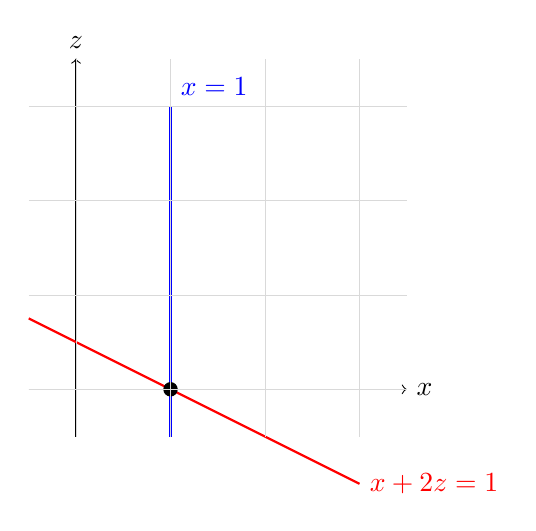
\begin{tikzpicture}[scale=1.2]
    % Axes
    \draw[->] (-0.5,0) -- (3.5,0) node[right] {$x$};
    \draw[->] (0,-0.5) -- (0,3.5) node[above] {$z$};
    
    % Lines
    \draw[thick,blue] (1,-0.5) -- (1,3) node[above right] {$x=1$};
    \draw[thick,red] (-0.5,0.75) -- (3, -1) node[right] {$x + 2 z = 1$};
    
    % Labels for intersection
    \filldraw[black] (1,0) circle (2pt) node[below right] {};
    
    % Optional grid
    \draw[very thin, gray!30] (-0.5,-0.5) grid (3.5,3.5);
\end{tikzpicture}

\textbf{Solution (3):}
The lines intersect at the $x$-axis because in the $xz$-plane the $x$-axis is defined by $z = 0$.

\subsection{Projective Changes of Coordinates}

\begin{tcolorbox}[title=Problem 1, breakable]
    For the complex affine change of coordinates 
    \[u = ax + by + e.\]
    \[v = cx + dy + f,\]
    where $a, b, c, d \in \mathbb{C}$ and $ad - bc \ne 0$, show that 
    \[u = ax + by + ez,\]
    \[v = cx + dy + fz,\]
    \[w = z,\]
    is the corresponding projective change of coordinates.
\end{tcolorbox}

\begin{proof}
    We have $\psi(u, v) = \left(\frac{ax + by + e}{z} : \frac{cx + dy + f}{z} : 1\right) = (ax + by + e : cx + dy + f : z)$.
\end{proof}

\begin{tcolorbox}[title=Problem 2, breakable]
    Let $C_1 = V(x^2 + y^2 - 1)$ be an ellipse in $\mathbb{C}^2$
        and let $C_2 = V(u^2 - v)$ be a parabola in $\mathbb{C}^2$.
    Homogenize the defining polynomials for $C_1$ and $C_2$ and show that 
        the projective change of coordinates 
    \[u = ix,\]
    \[v = y + z,\]
    \[w = y - z,\]
    transforms the ellipse in $\mathbb{P}^2$ into the parabola in $\mathbb{P}^2$.
\end{tcolorbox}

\begin{proof}
    We first homogenize $C_1$ and $C_2$ to obtain
    \[x^2 + y^2 - z^2 = 0 \quad \text{and} \quad u^2 - vw = 0.\]
    Then substituting our change of variables gives
    \[u^2 - vw = (ix)^2 - (y + z)(y - z)
    = -x^2 - (y^2 - z^2)
    = -(x^2 + y^2 - z^2) = 0,\]
    as required.
\end{proof}

\begin{tcolorbox}[title=Problem 3, breakable]
    Use the results of Section 1.3, together with the above problem,
        to show that, under a projective change of coordinates,
        all ellipses, hyperbolas, and parabolas are equivalent in $\mathbb{P}^2$.
\end{tcolorbox}


\begin{proof}
    By Section 1.3 ellipses and hyperbolas are equivalent under affine
    changes of coordinates, and by Problem 1 these extend to
    projective changes of coordinates in $\mathbb{P}^2$.
    By Problem 2 ellipses are equivalent to parabolas in $\mathbb{P}^2$.
    Therefore under a projective change of coordinates, all ellipses,
    hyperbolas, and parabolas are equivalent in $\mathbb{P}^2$.
\end{proof}

\subsection{The Complex Projective Line $\mathbb{P}^1$}

\begin{tcolorbox}[title=Problem 1, breakable]
    Suppose that $(x_1, y_1) \sim (x_2, y_2)$ and that $x_1 = x_2 \ne 0$.
    Show that $y_1 = y_2$.
\end{tcolorbox}

\begin{proof}
    We know there exists $\lambda$ such that $x_1 = \lambda x_2$.
    Dividing by $x_2 \ne 0$ shows $\lambda = 1$.
    But then $y_1 = \lambda y_2 = y_2$.
\end{proof}

\begin{tcolorbox}[title=Problem 2, breakable]
    Suppose that $(x_1, y_1) \sim (x_2, y_2)$ with $y_1 \ne 0$
    and $y_2 \ne 0$. Show that 
    \[(x_1, y_1) \sim \left(\frac{x_1}{y_1}, 1\right) = \left(\frac{x_2}{y_2}, 1\right) \sim (x_2, y_2).\]
\end{tcolorbox}


\begin{proof}
    Let $\lambda = y_1$ to see that 
    \[\left(\lambda \frac{x_1}{y_1}, \lambda \cdot 1\right) = (x_1, y_1).\]
    Thus $(x_1, y_1) \sim \left(\frac{x_1}{y_1}, 1\right)$.
    Similarly, $(x_2, y_2) \sim \left(\frac{x_2}{y_2}, 1\right)$.
    Since $(x_1, y_1) \sim (x_2, y_2)$ and $\sim$ is an equivalence relation
    \[
    \left(\frac{x_1}{y_1}, 1\right)
    =
    \left(\frac{x_2}{y_2}, 1\right).
    \]
\end{proof}

\begin{tcolorbox}[title=Problem 3, breakable]
    Explain why the elements of $\mathbb{P}^1$ can intuitively 
    be thought of as complex lines through the origin in $\mathbb{C}^2$.
\end{tcolorbox}

\textbf{Solution: } 
Take a line passing through the origin in $\mathbb{C}^2$
with direction vector $(a, b) \ne (0,0)$. 
This line consists of all points of the form $(\lambda a, \lambda b)$
 such that $\lambda \in \mathbb{C}$.
If we require $\lambda \ne 0$
we get the equivalence class $(a : b : c) \in \mathbb{P}^2$.
Thus each element of $\mathbb{P}^1$ represents a complex
    line through the origin in $\mathbb{C}^2$.

\begin{tcolorbox}[title=Problem 4, breakable]
    If $b \ne 0$, show that the line $x = \lambda a$, $y = \lambda b$ 
        will intersect the line $\{(x, y) \mid y = 1\}$ in exactly one point.
    Show that the point of intersection is $\left(\frac{a}{b}, 1\right)$.
\end{tcolorbox}

\begin{proof}
    We have $1 = y = \lambda b$ thus $\lambda = \frac{1}{b}$.
    Therefore $(x, y) = (\lambda a, 1) = \left(\frac{a}{b}, 1\right)$.
\end{proof}

\begin{tcolorbox}[title=Problem 5, breakable]
    Show that the map $\psi : \mathbb{C} \rightarrow \{(x : y) \in \mathbb{P}^2 \mid y \ne 0\}$
    defined by $\psi(x) = (x : 1)$ is a bijection.
\end{tcolorbox}

\begin{proof}
    Suppose $a, b \in \mathbb{C}$ such that $\psi(a) = \psi(b)$.
    Then 
    \[\psi(a) = \psi(b) \iff (a : 1) = (b : 1).\]
    But then since $1 = \lambda 1$ we have $\lambda = 1$ so $a = b$.
    Let $(a : y)$ be an arbitrary element in $\{(x : y) \in \mathbb{P}^2 \mid y \ne 0\}$.
    Then $(a : y) = \left(\frac{a}{y} : 1\right) = \psi\left(\frac{a}{b}\right)$.
    Thus $\psi$ is a bijection.
\end{proof}

\begin{tcolorbox}[title=Problem 6, breakable]
    Find a map $\{(x : y) \in \mathbb{P}^1 \mid y \ne 0\}$ to $\mathbb{C}$
    that is the inverse of the map $\psi$ in Exercise 1.6.5.
\end{tcolorbox}

\textbf{Solution:}
\[\psi^{-1}(x : y) = \frac{x}{y}.\]

\begin{tcolorbox}[title=Problem 7, breakable]
    Consider the map $\psi : \mathbb{C} \rightarrow \mathbb{P}^2$ given by 
    $\psi(x) = (x : 1)$. Show that as $|x| \rightarrow \infty$,
        we have $\psi(x) \rightarrow (1 : 0)$.
\end{tcolorbox}

\begin{proof}
    We have 
    \[(x : 1) = \left(1 : \frac{1}{x}\right).\]
    As $|x| \to \infty$, we have $\frac{1}{x} \to 0$ thus
    \[
    \left(1 : \frac{1}{x}\right) \to (1 : 0).
    \]
\end{proof}

\begin{tcolorbox}[title=Problem 8, breakable]
    Let $p$ denote the point $(0, 0, 1) \in S^2$, and let $l$
    denote the line through $p$ and the point $(x, y, 0)$
    in the $xy$-plane, whose parametrization is given by 
    \[\rho(t) = (1 - t)(0, 0, 1) + t(x, y, 0),\]
    i.e.,
    \[l = \{(tx, ty, 1 - t) \mid t \in \mathbb{R}\}.\]
    \begin{enumerate}
        \item $l$ clearly intersects $S^2$ at the point $p$. Show that there is exactly one other point of intersection $q$.
        \item Find the coordinates of $q$.
        \item Define the map $\psi : \mathbb{R}^2 \rightarrow S^2 - \{p\}$ to be the map that takes the point $(x, y)$ to the point $q$.
              Show that $\psi$ is a continuous bijection.
        \item Show that as $\sqrt{x^2 + y^2} \rightarrow \infty$, we have $\psi(x, y) \rightarrow p$. Thus as we move away from the origin 
                in $\mathbb{R}^2$, $\psi(x, y)$ moves toward the North Pole.
    \end{enumerate}
\end{tcolorbox}

\begin{proof}
    We substitute $l$ into the unit sphere equation to find 
    \[
    x^2 + y^2 + z^2 - 1 = (tx)^2 + (ty)^2 + (1 - t)^2 - 1 
    = t^2(x^2 + y^2 + 1) - 2t 
    = t \big( t(x^2 + y^2 + 1) - 2 \big) = 0.
    \]
    Now $t = 0$ corresponds to $p$. The other point corresponds to
    \[
    t(x^2 + y^2 + 1) - 2 = 0 \quad \implies \quad t = \frac{2}{x^2 + y^2 + 1}.
    \]
    Substituting back into the line gives
    \[
    q = \left( \frac{2x}{x^2 + y^2 + 1}, \frac{2y}{x^2 + y^2 + 1}, \frac{x^2 + y^2 - 1}{x^2 + y^2 + 1} \right).
    \]
\end{proof}

\begin{proof}
    Each coordinate is a continuous fraction thus $\psi$ is continuous.
    Suppose $(x, y), (a,b) \in \mathbb{R}^2$ such that 
    \[\psi(x, y) = \psi(a, b) 
        \iff \left( \frac{2x}{x^2 + y^2 + 1}, \frac{2y}{x^2 + y^2 + 1}, \frac{x^2 + y^2 - 1}{x^2 + y^2 + 1} \right) 
            = \left( \frac{2a}{a^2 + b^2 + 1}, \frac{2b}{a^2 + b^2 + 1}, \frac{a^2 + b^2 - 1}{a^2 + b^2 + 1} \right)\]
    From the third coordinate we infer $x^2 + y^2 + 1 = a^2 + b^2 + 1$.
    Then from the first coordinates we see $a = x$ and $b = y$.
    Thus $\psi$ is injective.
    Suppose $(X, Y, Z) \in S^2 - \{p\}$.
    We can solve the following equations for $x, y$
    \[\frac{2x}{x^2 + y^2 + 1} = X, \quad  \frac{2y}{x^2 + y^2 + 1} = Y, \quad  \frac{x^2 + y^2 - 1}{x^2 + y^2 + 1} = Z.\]
    Thus 
    \[x = \frac{X}{1 - Z} \quad \text{ and }  \quad y = \frac{Y}{1 - Z}.\]
    Finally, we see 
    \[\psi(x, y) = (X, Y, Z).\]
    Thus $\psi$ is surjective and it follows that $\psi$ is a bijection.
\end{proof}

\begin{proof}
    As $\sqrt{x^2 + y^2} \to \infty$ we have 
        $\frac{2x}{x^2 + y^2 + 1} \to 0$,
        $\frac{2y}{x^2 + y^2 + 1} \to 0$, and 
        $\frac{x^2 + y^2 - 1}{x^2 + y^2 + 1} \to 1$.
    Thus $q \to (0, 0, 1) = p$.
\end{proof}

\begin{tcolorbox}[title=Problem 9, breakable]
    Determine which point(s) in $\mathbb{P}^1$ do \textbf{not}
    have two representitives of the form $(x : 1) = (1 : \frac{1}{x})$.
\end{tcolorbox}

\textbf{Solution: }
\[(0 : 1) \in \mathbb{P}^1.\]

\begin{tcolorbox}[title=Problem 10, breakable]
    Map $U \rightarrow \mathbb{P}^1$ via $x \mapsto (x : 1)$
        and map $V \rightarrow \mathbb{P}^1$ via $y \mapsto (1 : y)$.
    Show that $(x : 1) \mapsto \left(1 : \frac{1}{x}\right)$ is a natural one-to-one 
    map from $U^*$ to $V^*$.
\end{tcolorbox}

\begin{proof}
    Let $x, y \in U^*$ then under the map we have $\left(1 : \frac{1}{x}\right) = \left(1 : \frac{1}{y}\right) \in V^*$.
    Then since $1$ is the first coordinate we have $\lambda = 1$ thus $x = y$.
    Therefore the mapping is a natural one-to-one map from $U^*$ to $V^*$.
\end{proof}

\begin{tcolorbox}[title=Problem 11, breakable]
    A sphere can be split into a neighborhood of its northern hemisphere
        and a neighborhood of its southern hemisphere.
    Show that a sphere can be obtained by correctly gluing together two copies of $\mathbb{C}$.
\end{tcolorbox}

\begin{proof}
    We take two spaces $\mathbb{C}_1, \mathbb{C}_2$.
    Then define maps $\psi_1 : \mathbb{C}_1 \rightarrow \mathbb{R}^3 - \{0, 0, 1\}$, $\psi_2 : \mathbb{C}_2 \rightarrow \mathbb{R}^3 - \{0, 0, -1\}$ by
    \[
    \psi_1(x, y) = \left( \frac{2x}{x^2 + y^2 + 1}, \frac{2y}{x^2 + y^2 + 1}, \frac{x^2 + y^2 - 1}{x^2 + y^2 + 1} \right),
    \]
    and 
    \[
    \psi_2(u, v) = \left( \frac{2u}{u^2 + v^2 + 1}, \frac{2v}{u^2 + v^2 + 1}, \frac{1 - u^2 - v^2}{u^2 + v^2 + 1} \right).
    \]
    Then
    \[
    S^2 = \psi_1(\mathbb{C}_1) \cup \psi_2(\mathbb{C}_2).
    \]
\end{proof}

\begin{tcolorbox}[title=Problem 12, breakable]
    Put together the last two exercises to show that $\mathbb{P}^1$ is topologically equivalent 
        to a sphere.
\end{tcolorbox}

\begin{proof}
    From Problem 10, we can map the two spaces $U^*$ and $V^*$ to $\mathbb{P}^1$.
    We can then equate $U^*$ and $V^*$ to the two copies of $\mathbb{C}$.
    Then from Problem 11 there is a homeomorphism from the two spaces $\mathbb{C}$ to $S^2$.
    Thus $\mathbb{P}^1$ is homeomorphic to $S^2$.
\end{proof}

\subsection{Ellipses, Hyperbolas, and Parabolas as Spheres}

\begin{tcolorbox}[title=Problem 1, breakable]
    Find a bijective polynomial map from $\mathbb{C}$ to the conic 
    $C = \{(x, y) \in \mathbb{C}^2 \mid x^2 - y = 0\}$
\end{tcolorbox}

\begin{proof}
    We first paramtrize $C$ as follows 
    \[x = t \text{ and } y = t^2.\]
    Then, we define the mapping $\psi : \mathbb{C} \rightarrow C$ as 
    \[\psi(\alpha) = (\alpha, \alpha^2).\]
    Now, suppose $\alpha_1, \alpha_2 \in \mathbb{C}$ and $\psi(\alpha_1) = \psi(\alpha_2)$. Then 
    \[\psi(\alpha_1) = \psi(\alpha_2) \iff (\alpha_1, \alpha_1^2) = (\alpha_2, \alpha_2^2) \iff \alpha_1 = \alpha_2.\]
    Thus $\psi$ is injective.
    Now, let $(x, y) \in C$ and notice $y = x^2$.
    Then $\psi(x) = (x, x^2) = (x, y)$.
    Thus $\psi$ is surjective.
    It follows that $\psi$ is a bijection from $\mathbb{C}$ to $C$.
\end{proof}

\begin{tcolorbox}[title=Problem 2, breakable]
    Let $C = V(x^2 + y^2 - 1)$ be an ellipse in $\mathbb{C}^2$.
    Find a trigonometric parametrization of $C$.
    [Hint: Think high school trigonometry.]
\end{tcolorbox}

\begin{proof}
    Let $x = \cos(t)$ and $y = \sin(t)$ for $t \in \mathbb{C}$.
\end{proof}

\begin{tcolorbox}[title=Problem 3, breakable]
    Consider the ellipse $C = V(x^2 + y^2 - 1) \subset \mathbb{C}^2$
    and let $p$ denote the point $(0, 1) \in C$.
    \begin{enumerate}
        \item Parametrize the line segment from $p$ to the point $(\lambda, 0)$ on 
                the complex line $y = 0$ as in Exercise 16.8.
        \item This line segment clearly intersects $C$ at the point $p$. Show 
                that if $\lambda \ne \pm i$, then there is exactly one other point 
                of intersection. Call this point $q$.
        \item Find the coordinates of $q \in C$.
        \item Show that if $\lambda = \pm i$, then the line segment intersects $C$ only at $p$.
    \end{enumerate}
\end{tcolorbox}

\begin{proof}
    We have $p + x(p - (\lambda, 0))$ for $x \in \mathbb{C}$.
    Then 
    \[p + x(p - (\lambda, 0)) = (0, 1) + x((0, 1) - (\lambda, 0)) = (0, 1) + x(-\lambda, 1) = (-\lambda x, 1 + x).\]
\end{proof}

\begin{proof}
    Suppose $\lambda \ne \pm i$.
    Then 
    \[
        (-\lambda x)^2 + (1 + x)^2 - 1 
        = \lambda^2 x^2 + (1 + 2x + x^2) - 1 
        = (\lambda^2 + 1)x^2 + 2x 
        = x\big((\lambda^2 + 1)x + 2\big) = 0.
    \]
    $x = 0$ corresponds to $p$.  
    \[
        x = -\frac{2}{\lambda^2 + 1}
    \]
    corresponds to 
    \[
        q = \left(-\lambda\!\left(-\frac{2}{\lambda^2 + 1}\right),\, 1 - \frac{2}{\lambda^2 + 1}\right).
    \]
\end{proof}

\begin{proof}
    Suppose $\lambda = \pm i$.
    Then 
    \[
        (-\lambda x)^2 + (1 + x)^2 - 1 = (-(\pm i) x)^2 + (1 + 2x + x^2) - 1 = 2x = 0.
    \]
    $x = 0$ corresponds to $p$ and there are no other solutions.
\end{proof}

\begin{tcolorbox}[title=Problem 4, breakable]
    Define the map $\tilde{\psi} : \mathbb{C} \rightarrow C \subset \mathbb{C}^2$ by
    \[\tilde{\psi}(\lambda) = \left(\frac{2 \lambda}{\lambda^2 + 1}, \frac{\lambda^2 - 1}{\lambda^2 + 1}\right).\]
    Show that the above map can be extended to the map 
    \[\psi : \mathbb{P}^1 \rightarrow \{(x : y : z) \in \mathbb{P}^2 \mid x^2 + y^2 - z^2 = 0\}.\]
    given by 
    \[\psi(\lambda : u) = (2 \lambda u : \lambda^2 - u^2 : \lambda^2 + u^2).\]
\end{tcolorbox}

\begin{proof}
    Plugging in we find 
    \begin{align*}
        (2\lambda u)^2 + (\lambda^2 - u^2)^2 - (\lambda^2 + u^2)^2
        &= 4\lambda^2 u^2 + (\lambda^4 - 2\lambda^2 u^2 + u^4)
           - (\lambda^4 + 2\lambda^2 u^2 + u^4) \\
        &= 4\lambda^2 u^2 + \lambda^4 - 2\lambda^2 u^2 + u^4
           - \lambda^4 - 2\lambda^2 u^2 - u^4 \\
        &= 0.
    \end{align*}
\end{proof}

\begin{tcolorbox}[title=Problem 5, breakable]
    \begin{enumerate}
        \item Show that the map $\psi$ is one-to-one.
        \item Show that $\psi$ is onto. [Hint: Consider the two cases: $z \ne 0$ and $z = 0$.
                For $z \ne 0$ follow the contruction given above. For $z = 0$, find values of 
                $\lambda$ and $u$ to show that these points are given by $\psi$. How does this 
                relate to Part 4 of Exercise 1.7.3?]
    \end{enumerate}
\end{tcolorbox}

\begin{proof}
    Let $(\lambda : u), (\lambda' : u') \in \mathbb{P}^1$. Then 
    \[
        \psi(\lambda : u) = \psi(\lambda' : u') 
        \iff 
        (2 \lambda u : \lambda^2 - u^2 : \lambda^2 + u^2) 
        = 
        (2 \lambda' u' : \lambda'^2 - u'^2 : \lambda'^2 + u'^2).
    \]
    There exists $k \in \mathbb{C}$ such that 
    \[
        2 \lambda u = k(2 \lambda' u'), \quad 
        \lambda^2 - u^2 = k(\lambda'^2 - u'^2) = k \lambda'^2 - k u'^2, \quad  
        \lambda^2 + u^2 = k(\lambda'^2 + u'^2) = k \lambda'^2 + k u'^2.
    \]
    Adding the second and third equations shows 
    \[\lambda^2 = k \lambda'^2.\]
    Subtracting the second and third equations shows 
    \[-2 u^2 = - 2 k u'^2 \implies u^2 = k u'^2.\]
    Thus $(\lambda : u) = (\lambda' : u')$ in $\mathbb{P}^1$.
    It follows that $\psi$ is injective.

    Suppose $z = 0$. We have 
    \[x^2 + y^2 - z^2 = 0 \iff -x^2 = y^2 \iff y = \pm i x.\]
    Then 
    \[(x : \pm i x : z) = (1 : \pm i : 0).\]
    We have 
    \[\lambda^2 + u^2 = 0 \iff \lambda^2 = - u^2 \iff \lambda = \pm i u.\]
    Then 
    \[\psi(\pm i u : u) = (2 (\pm i u) u : (\pm i u)^2 - u^2 : (\pm i u)^2 + u^2)  = (\pm 2 i u^2 : -2 u^2 : 0) = (1 : \pm i : 0).\]

    Now, suppose $z \ne 0$.
    Let $(x : y : z)$ be an element in $\mathbb{P}^2$ with $z \ne 0$.
    We require 
    \[2 \lambda u = x, \quad \lambda^2 - u^2 = y, \quad \lambda^2 + u^2 = z.\]
    Adding and subtracting the second and third equations we find 
    \[\lambda^2 = \frac{y + z}{2} \implies \lambda = \pm \sqrt{\frac{y + z}{2}}, \quad u^2 = \frac{z - y}{2} \implies u = \pm \sqrt{\frac{z - y}{2}}.\]
    Then 
    \[\psi\left(\pm \sqrt{\frac{y + z}{2}}, \pm \sqrt{\frac{z - y}{2}}\right) = (x : y : z).\]
    Thus $\psi$ is surjective.
\end{proof}

\begin{tcolorbox}[title=Problem 6, breakable]
    For the following conics and the given point $p$, follow 
    what we did for the conic $x^2 + y^2 - 1 = 0$ to find a rational 
    map from $\mathbb{C}$ to the curve $\mathbb{C}^2$ and then a one-to-one 
    map from $\mathbb{P}^1$ onto the conic in $\mathbb{P}^2$.
    \begin{enumerate}
        \item $x^2 + 2x - y^2 - 4y - 4 = 0$ with $p = (0, -2)$.
        \item $3x^2 + 3y^2 - 75 = 0$ with $p = (5, 0)$.
        \item $4x^2 + y^2 - 8 = 0$ with $p = (1, 2)$.
    \end{enumerate}
\end{tcolorbox}

\textbf{Solution (1): }
Consider the line $y = mx - 2$. We have 
\begin{align*}
x^2 + 2x - y^2 - 4y - 4 &= 0 \\
&\iff x^2 + 2x - (mx - 2)^2 - 4(mx - 2) - 4 = 0 \\
&\iff x^2 + 2x - (m^2x^2 - 4mx + 4) - 4mx + 8 - 4 = 0 \\
&\iff (1 - m^2)x^2 + 2x = 0 \\ 
&\iff x[(1 - m^2)x + 2] = 0.
\end{align*}
Then $x = 0$ corresponds to $p$.
So $x = \frac{-2}{1 - m^2}$, thus $y = \frac{-2m - 2(1 - m^2)}{1 - m^2}$.
So we have the parametrization 
\[
x(m) = \frac{-2}{1 - m^2}, \quad y(m) = \frac{2m^2 - 2m - 2}{1 - m^2}.
\]
Then define $\psi : \mathbb{P}^1 \rightarrow \mathbb{P}^2$ as
\[
\psi(m, u) = (-2 : 2m^2 - 2m - 2 : 1 - m^2).
\]

\textbf{Solution (2):}
Consider the line $y = m(x - 5) = mx - 5m$. We have 
\begin{align*}
3x^2 + 3y^2 - 75 &= 0 \\
&\iff 3x^2 + 3(mx - 5m)^2 - 75 = 0 \\
&\iff 3x^2 + 3(m^2x^2 - 10m^2x + 25m^2) - 75 = 0 \\
&\iff 3x^2 + 3m^2x^2 - 30m^2x + 75m^2 - 75 = 0 \\
&\iff 3(1 + m^2)x^2 - 30m^2x + 75(m^2 - 1) = 0 \\
&\iff (1 + m^2)x^2 - 10m^2x + 25(m^2 - 1) = 0 \\
&\iff [(1 + m^2)x - 5(m^2 + 1)][x - 5] = 0.
\end{align*}
Then $x = 5$ corresponds to $p$.
So $x = \frac{5(m^2 + 1)}{1 + m^2} = 5$, thus $y = m(x - 5) = m(5 - 5) = 0$.
So we have the parametrization 
\[
x(m) = 5, \quad y(m) = 0.
\]
Then define $\psi : \mathbb{P}^1 \rightarrow \mathbb{P}^2$ as
\[
\psi(m, u) = (5 : 0 : 1).
\]

\textbf{Solution (3):}
Consider the line $y = m(x - 1) + 2 = mx - m + 2$. We have 
\begin{align*}
4x^2 + y^2 - 8 &= 0 \\
&\iff 4x^2 + (mx - m + 2)^2 - 8 = 0 \\
&\iff 4x^2 + (m^2x^2 - 2m^2x + 4mx + m^2 - 4m + 4) - 8 = 0 \\
&\iff (4 + m^2)x^2 + (-2m^2 + 4m)x + (m^2 - 4m - 4) = 0 \\
&\iff (x - 1)\big((4 + m^2)x + (-4 + m^2 + 4m)\big) = 0.
\end{align*}
Then $x = 1$ corresponds to $p$.
So $x = \frac{4 - m^2 - 4m}{4 + m^2}$, thus 
\[
y = m\left(\frac{4 - m^2 - 4m}{4 + m^2} - 1\right) + 2.
\]
So we have the parametrization 
\[
x(m) = \frac{4 - m^2 - 4m}{4 + m^2}, \quad y(m) = m\left(\frac{4 - m^2 - 4m}{4 + m^2} - 1\right) + 2.
\]
Then define $\psi : \mathbb{P}^1 \rightarrow \mathbb{P}^2$ as
\[
\psi(m, u) = (4 - m^2 - 4m : m(4 - m^2 - 4m - (4 + m^2)) + 2(4 + m^2) : 4 + m^2).
\]

\subsection{Links to Number Theory}

\begin{tcolorbox}[title=Problem 1, breakable]
    Suppose $(x_0, y_0, z_0)$ is a solution to $x^2 + y^2 = z^2$.
    Show that $(m x_0, m y_0, m z_0)$ is also a solution for any scalar $m$.
\end{tcolorbox}

\begin{proof}
    We have 
    \[
        x_0^2 + y_0^2 - z_0^2 
            = 0 \iff m^2(x_0^2 + y_0^2 - z_0^2) 
            = 0 \iff m^2 x_0^2 + m^2 y_0^2 - m^2 z_0^2 
            = 0 \iff (mx_0)^2 + (my_0)^2 - (mz_0)^2 = 0.
    \]
    Thus $(m x_0, m y_0, m z_0)$ is also a solution for any scalar $m$.
\end{proof}

\begin{tcolorbox}[title=Problem 2, breakable]
    Let $(a, b, c) \in \mathbb{Z}^3$ be a solution to $x^2 + y^2 = z^2$.
    Show that $c = 0$ if and only if $a = b = 0$.
\end{tcolorbox}

\begin{proof}
    Suppose $c = 0$ then clearly $a = b = 0$.
    Suppose $a = b = 0$. Then 
    $a^2 + b^2 = 0^2 + 0^2 = 0$.
    Thus $c = 0$.
\end{proof}

\begin{tcolorbox}[title=Problem 3, breakable]
    Show that if $(a, b, c)$ is a Pythagorean triple with $c \ne 0$,
    then the pair of rational number $\left(\frac{a}{c}, \frac{b}{c}\right)$
    is a solution to $x^2 + y^2 = 1$.
\end{tcolorbox}

\begin{proof}
    Suppose $(a, b, c)$ is a Pythagorean triple with $c \ne 0$.
    Then 
    \[a^2 + b^2 = c^2 \iff \frac{a^2}{c^2} + \frac{b^2}{c^2} = 1 \iff \left(\frac{a}{c}\right)^2 + \left(\frac{b}{c}\right)^2 = 1.\]
\end{proof}

\begin{tcolorbox}[title=Problem 4, breakable]
    Let $\left( \frac{a}{c_1}, \frac{b}{c_2} \right) \in \mathbb{Q}^2$ be a rational solution to 
    $x^2 + y^2 = 1$. Find a corresponding Pythagorean triple.
\end{tcolorbox}

\begin{proof}
    First, write $\frac{a}{c_1}, \frac{b}{c_2}$ in their lowest terms by dividing by common factors.
    Then 
    \[
        \left(\frac{a}{c_1}\right)^2 + \left(\frac{b}{c_2}\right)^2 = 1 
        \iff (a c_2)^2 + (b c_1)^2 = (c_1 c_2)^2.
    \]
    Thus $(a c_2, b c_1, c_1 c_2)$ is a Pythagorean triple.
\end{proof}

\begin{tcolorbox}[title=Problem 5, breakable]
    Let
    \[C(\mathbb{Q}) = \{(x, y) \in \mathbb{Q}^2 \mid x^2 + y^2 = 1\}.\]
    Define the map $\tilde{\psi} : \mathbb{Q} \rightarrow \{(x, y) \in \mathbb{Q}^2 \mid x^2 + y^2 = 1\}.$ as 
    \[\lambda \mapsto \left(\frac{2 \lambda}{\lambda^2 + 1}, \frac{\lambda^2 - 1}{\lambda^2 + 1}\right).\]
    Show that the above map $\tilde{\psi}$ sends $\mathbb{Q} \rightarrow C(\mathbb{Q})$.
\end{tcolorbox}

\begin{proof}
    Let $\lambda \in \mathbb{Q}$
    Then $\tilde{\lambda} = \left(\frac{2 \lambda}{\lambda^2 + 1}, \frac{\lambda^2 - 1}{\lambda^2 + 1}\right)$.
    Plugging in we find 
    \begin{align*}
        \left(\frac{2 \lambda}{\lambda^2 + 1}\right)^2 + \left( \frac{\lambda^2 - 1}{\lambda^2 + 1}\right)^2 
        &= \frac{4 \lambda^2}{(\lambda^2 + 1)^2} + \frac{(\lambda^2 - 1)^2}{(\lambda^2 + 1)^2} \\
        &= \frac{4 \lambda^2 + (\lambda^4 - 2 \lambda^2 + 1)}{(\lambda^2 + 1)^2} \\
        &= \frac{\lambda^4 + 2 \lambda^2 + 1}{(\lambda^2 + 1)^2} \\
        &= 1.
    \end{align*}
\end{proof}

\begin{tcolorbox}[title=Problem 6, breakable]
    \begin{enumerate}
        \item Show that $\psi : \mathbb{P}^1(\mathbb{Q}) \rightarrow C(\mathbb{Q}) \subset \mathbb{P}^2(\mathbb{Q})$ is onto.
        \item Show that every primitive triple is of the form $(2 \lambda u, \lambda^2 - u^2, \lambda^2 + u^2)$.
    \end{enumerate}
\end{tcolorbox}

\begin{proof}
    This is the same as 1.7.5.
    $\psi$ is a bijection thus every primitive triple is of that form.
\end{proof}

\begin{tcolorbox}[title=Problem 7, breakable]
    Find a rational point on the conic $x^2 + y^2 - 2 = 0$.
    Develop a parametrization and conclude that there are infinitely many rational points on this curve.
\end{tcolorbox}

\begin{proof}
    Consider $p = (1, 1) \in \mathbb{Q}^2$.
    Then $x^2 + y^2 - 2 = 1 + 1 - 2 = 0$.
    Consider the line $y = m(x - 1) + 1 = mx - m + 1$.
    Then 
    \begin{align*}
    x^2 + (mx - m + 1)^2 - 2 
    &= x^2 + \big(mx - m + 1\big)^2 - 2 \\
    &= x^2 + \big(m^2 x^2 - 2 m^2 x + 2 m x + m^2 - 2 m + 1\big) - 2 \\
    &= (1 + m^2)x^2 + 2 m (1 - m)x + (m^2 - 2 m - 1) \\
    &= (x - 1)\big((1 + m^2)x - m^2 + 2 m + 1\big)
    \end{align*}
    Now, $x = 1$ corresponds to $p$.
    So we have $x = \frac{m^2 - 2m - 1}{1 + m^2}$.
    Then we have the paramtrization 
    \[x(m) = \frac{m^2 - 2m - 1}{1 + m^2}, \quad y(m) = m\left(\frac{m^2 - 2m - 1}{1 + m^2}\right) - m + 1.\]
    From this we can obtain infinitely many rational points on the curve.
\end{proof}

\begin{tcolorbox}[title=Problem 8, breakable]
    By mimicking the above, find four rational points on each of the following conics.
    \begin{enumerate}
        \item $x^2 + 2x - y^2 - 4y - 4 = 0$ with $p = (0, -2)$.
        \item $3x^ + 3y^2 - 75 = 0$ with $p = (5, 0)$.
        \item $4 x^2 + y^2 - 8 = 0$ with $p = (1, 2)$.
    \end{enumerate}
\end{tcolorbox}

\begin{proof}
    \textbf{(1)} Consider $p = (0, -2) \in \mathbb{Q}^2$.
    Then $x^2 + 2x - y^2 - 4y - 4 = 0$ at $(0, -2)$.
    Consider the line $y = m(x - 0) - 2 = mx - 2$.
    Then 
    \begin{align*}
    x^2 + 2x - (mx - 2)^2 - 4(mx - 2) - 4
    &= x^2 + 2x - (m^2 x^2 - 4 m x + 4) - (4 m x - 8) - 4 \\
    &= (1 - m^2)x^2 + (2 + 0)x + (-4 + 8 - 4) \\
    &= (1 - m^2)x^2 + 2 x + 0 \\
    &= x\big((1 - m^2)x + 2\big)
    \end{align*}
    Now, $x = 0$ corresponds to $p$.
    So we have $x = \frac{-2}{1 - m^2}$.
    Then we have the parametrization 
    \[x(m) = \frac{-2}{1 - m^2}, \quad y(m) = m\left(\frac{-2}{1 - m^2}\right) - 2.\]
    From this we can obtain infinitely many rational points on the curve.
\end{proof}

\begin{proof}
    Consider $p = (5, 0) \in \mathbb{Q}^2$.
    Then $3x^2 + 3y^2 - 75 = 0$ at $(5, 0)$.
    Consider the line $y = m(x - 5) + 0 = m(x - 5)$.
    Then
    \begin{align*}
    3x^2 + 3(mx - 5m)^2 - 75
    &= 3x^2 + 3(m^2 x^2 - 10 m^2 x + 25 m^2) - 75 \\
    &= 3(1 + m^2)x^2 - 30 m^2 x + 75(m^2 - 1) \\
    &= (x - 5)\big(3(1 + m^2)x - 30 m^2 - 75\big)
    \end{align*}
    Now, $x = 5$ corresponds to $p$.
    So the other intersection point satisfies
    \[
        3(1 + m^2)x - 30 m^2 - 75 = 0 \implies x = \frac{30 m^2 + 75}{3(1 + m^2)} = \frac{10 m^2 + 25}{1 + m^2}.
    \]
    Then we have the parametrization
    \[
        x(m) = \frac{10 m^2 + 25}{1 + m^2}, \quad y(m) = m\left(\frac{10 m^2 + 25}{1 + m^2} - 5\right) = m\left(\frac{10 m^2 + 25 - 5 - 5 m^2}{1 + m^2}\right) = m\left(\frac{5 m^2 + 20}{1 + m^2}\right).
    \]
    From this we can obtain infinitely many rational points on the curve.
\end{proof}

\begin{proof}
    Consider $p = (1, 2) \in \mathbb{Q}^2$.
    Then $4x^2 + y^2 - 8 = 0$ at $(1, 2)$.
    Consider the line $y = m(x - 1) + 2 = mx - m + 2$.
    Then 
    \begin{align*}
    4x^2 + (mx - m + 2)^2 - 8
    &= 4x^2 + (m^2 x^2 - 2 m^2 x + 2 m x + m^2 - 4 m + 4) - 8 \\
    &= (4 + m^2)x^2 + 2 m(1 - m)x + (m^2 - 4 m - 4) \\
    &= (x - 1)\big((4 + m^2)x + 2 m (1 - m) + (m^2 - 4 m - 4)\big)
    \end{align*}
    Now, $x = 1$ corresponds to $p$.
    So we have $x = \frac{-2 m^2 + 2 m + 4}{4 + m^2}$.
    Then we have the parametrization 
    \[x(m) = \frac{-2 m^2 + 2 m + 4}{4 + m^2}, \quad y(m) = m\left(\frac{-2 m^2 + 2 m + 4}{4 + m^2} - 1\right) + 2.\]
    From this we can obtain infinitely many rational points on the curve.
\end{proof}


\begin{tcolorbox}[title=Problem 9, breakable]
    Show that the conic $x^2 + y^2 = 3$ has no rational points.
\end{tcolorbox}

\begin{proof}
    Suppose $x = \frac{a}{b}$ and $y = \frac{c}{d}$ are in lowest terms with $a, b, c, d \in \mathbb{Z}$.
    Furthermore, suppose
    \[
        \left(\frac{a}{b}\right)^2 + \left(\frac{c}{d}\right)^2 = 3.
    \]
    Then
    \[
        \left(\frac{a}{b}\right)^2 + \left(\frac{c}{d}\right)^2 = 3
        \iff a^2 d^2 + c^2 b^2 = 3 b^2 d^2
        \iff (ad)^2 = 3 (bd)^2 - (bc)^2 = b^2(3d^2 - c^2).
    \]
    Now we must have $3d^2 - c^2 = k^2$ for some $k \in \mathbb{Z}$.
    We see $3d^2 - c^2 \equiv 0, 2 \pmod{3}$ while $k^2 \equiv 0, 1 \pmod{3}$.
    But, $\gcd(c, d) = 1$ thus $3d^2 - c^2 \equiv 2 \pmod{3}$ while $k^2 \equiv 0, 1 \pmod{3}$ which is a contradiction.
\end{proof}

\subsection{Degenerate Conics}

\begin{tcolorbox}[title=Problem 1, breakable]
    Dehomogenize $f(x, y, z)$ by setting $z = 1$. Graph 
    the curve 
    \[C(\mathbb{R}) = \{(x : y : z) \in \mathbb{P}^2 \mid f(x, y, 1) = 0\}.\]
    in the real plane $\mathbb{R}^2$.
\end{tcolorbox}

\begin{figure}[h!]
    \centering
    \includegraphics[width=0.3\textwidth]{images/chapter1/10.png}
\end{figure}

\begin{tcolorbox}[title=Problem 2, breakable]
    Consider the two lines given by 
    \[(a_1 x + b_1 y + c_1 z)(a_2 x + b_2 y + c_2 z) = 0,\]
    and suppose 
    \[\det \begin{bmatrix}
        a_1 & b_1 \\
        a_2 & b_2
    \end{bmatrix} \ne 0.\]
    Show that the two lines intersect at a point where $z \ne 0$.
\end{tcolorbox}

\begin{proof}
    Suppose the two lines intersect at a point where $z = 0$. Thus 
    \[
        a_1 x + b_1 y = 0
        \quad \text{and} \quad
        a_2 x + b_2 y = 0,
    \]
    so
    \[\begin{bmatrix}
        a_1 & b_1 \\
        a_2 & b_2
    \end{bmatrix} \begin{bmatrix}
        x \\
        y
    \end{bmatrix} = 0.\]
    Then 
    \[\det \begin{bmatrix}
        a_1 & b_1 \\
        a_2 & b_2
    \end{bmatrix} \ne 0 \implies \begin{bmatrix}
        x \\ y
    \end{bmatrix} = \begin{bmatrix}
        0 \\ 0
    \end{bmatrix}.\]
    Thus $x = y = 0$ but $(0, 0, 0) \notin \mathbb{P}^2$.
\end{proof}

\begin{tcolorbox}[title=Problem 3, breakable]
    Dehomogenize the equation in the previous exercise 
    by setting $z = 1$. Given an argument that, as lines in the 
    complex plane $\mathbb{C}^2$, they have distinct slopes.
\end{tcolorbox}

\begin{proof}
    Dehomogenizing we find 
    \[(a_1 x + b_1 y + c_1)(a_2 x + b_2 y + c_2) = 0.\]
    Since they intersect at a point such that $z \ne 0$ 
        they are not parallel in $\mathbb{C}^2$.
    Thus either $a_1 \ne a_2$ or $b_1 \ne b_2$.
\end{proof}

\begin{tcolorbox}[title=Problem 4, breakable]
    Again consider the two lines 
    \[(a_1 x + b_1 y + c_1 z)(a_2 x + b_2 y + c_2 z) = 0.\]
    Suppose that 
    \[\det \left( A = \begin{bmatrix}
        a_1 & b_1 \\
        a_2 & b_2
    \end{bmatrix} \right) = 0.\]
    but that 
    \[\det \begin{bmatrix}
        a_1 & c_1 \\
        a_2 & c_2
    \end{bmatrix} \ne 0 \text{ or } \begin{bmatrix}
        b_1 & c_1 \\
        b_2 & c_2
    \end{bmatrix} \ne 0.\]
    Show that the two lines still have one common point 
    of intersection but that this point must have $z = 0$.
\end{tcolorbox}

\begin{proof}
    Suppose the two lines intersect at a point such that $z \ne 0$.
    Then dividing by $z$ we find 
    \[\left(a_1 \frac{x}{z} + b_1 \frac{y}{z} + c_1\right)\left(a_2 \frac{x}{z} + b_2 \frac{y}{z} + c_2\right) = 0.\]
    Let $X = \frac{x}{z}, Y =\frac{y}{z}$.
    We now have the following system 
    \[\begin{bmatrix}
        a_1 & b_1 \\
        a_2 & b_2
    \end{bmatrix} \begin{bmatrix}
        X \\
        Y
    \end{bmatrix} = 
    \begin{bmatrix}
        -c_1 \\
        -c_2
    \end{bmatrix}.\]
    Since $\det(A) = 0$ the system does not have a unique solution.
    It follows that the lines are linearly dependent.
    Now, wlog suppose 
    \[\det \begin{bmatrix}
        a_1 & c_1 \\
        a_2 & c_2
    \end{bmatrix} \ne 0.\]
    Then $a_1 c_2 \ne a_2 c_1$ and it follows that the lines are not equivalent.
    Therefore, the lines are parallel and meet at $z = 0$.
\end{proof}

\begin{tcolorbox}[title=Problem 5, breakable]
    Let 
    \[f(x, y, z) = (a_1 x + b_1 y + c_1 z)(a_2 x + b_2 y + c_2 z),\]
    where at least one of $a_1, b_2$, or $c_1$ is non-zero and at least one 
    of the $a_2, b_2$, or $c_2$ is non-zero. Show that the curve defined 
    by $f(x, y, z) = 0$ is a double line if and only if 
    \[\det \begin{bmatrix}
        a_1 & b_1 \\
        a_2 & b_2
    \end{bmatrix} = 0, \quad \det \begin{bmatrix}
        a_1 & c_1 \\
        a_2 & c_2
    \end{bmatrix} = 0, \quad  \det \begin{bmatrix}
        b_1 & c_1 \\
        b_2 & c_2
    \end{bmatrix} = 0.\]
\end{tcolorbox}

\begin{proof}
    Suppose $f(x, y, z) = 0$ is a double line.  
    By Problem 4 we know
    \[
    \det \begin{bmatrix} a_1 & b_1 \\ a_2 & b_2 \end{bmatrix} = 0, \quad
    \det \begin{bmatrix} a_1 & c_1 \\ a_2 & c_2 \end{bmatrix} = 0, \quad
    \det \begin{bmatrix} b_1 & c_1 \\ b_2 & c_2 \end{bmatrix} = 0.
    \]
    Conversely, suppose
    \[
    \det \begin{bmatrix} a_1 & b_1 \\ a_2 & b_2 \end{bmatrix} = 0, \quad
    \det \begin{bmatrix} a_1 & c_1 \\ a_2 & c_2 \end{bmatrix} = 0, \quad
    \det \begin{bmatrix} b_1 & c_1 \\ b_2 & c_2 \end{bmatrix} = 0.
    \]  
    Thus $(a_2, b_2, c_2)$ is a scalar multiple of $(a_1, b_1, c_1)$.
    Therefore $f(x, y, z) = 0$ is a double line.
\end{proof}

\begin{tcolorbox}[title=Problem 6, breakable]
    Consider 
    \[(a_1 x + b_1 y + c_1 z)(a_2 x + b_2 y + c_2 z) = 0,\]
    with 
    \[\det \begin{bmatrix}
        a_1 & b_1 \\
        a_2 & b_2
    \end{bmatrix} \ne 0.\]
    Find a projective change of coordinates from $xyz$-space to $uvw$-space 
    so that the crossing lines become 
    \[uv = 0.\]
\end{tcolorbox}

\begin{proof}
    Consider
    \[
        u = a_1 x + b_1 y + c_1 z, \quad
        v = a_2 x + b_2 y + c_2 z, \quad
        w = z.
    \]
    Then,
    \[
        (a_1 x + b_1 y + c_1 z)(a_2 x + b_2 y + c_2 z)
        =
        uv.
    \]
\end{proof}

\begin{tcolorbox}[title=Problem 7, breakable]
    Consider the crossing lines $(a_2 x + b_1 y + c_1 z)(a_2 x + b_2 y + c_2 z) = 0$, with 
    \[\det \begin{bmatrix}
        a_1 & c_1 \\
        a_2 & c_2
    \end{bmatrix} \ne 0.\]
    Find a projective change of coordinates from $xyz$-space to $uvw$-space 
    so that the crossing lines become 
    \[uv = 0.\]
\end{tcolorbox}

\begin{proof}
    Consider
    \[
        u = a_1 x + b_1 y + c_1 z, \quad
        v = a_2 x + b_2 y + c_2 z, \quad
        w = z.
    \]
    Then,
    \[
        (a_1 x + b_1 y + c_1 z)(a_2 x + b_2 y + c_2 z)
        =
        uv.
    \]
\end{proof}

\begin{tcolorbox}[title=Problem 8, breakable]
    Show that there is a projective change of coordinates from $xyz$-space to $uvw$-space so that 
    the double lines $(ax + by + cz)^2 = 0$ becomes the double line
    \[u^2 = 0.\]
\end{tcolorbox}

\begin{proof}
    Consider
    \[
        u = a x + b y + c z, \quad
        v = a x + b y + c z, \quad
        w = z.
    \]
    Then,
    \[
        (a x + b y + c z)(a x + b y + c z)
        =
        u^2.
    \]
\end{proof}

\begin{tcolorbox}[title=Problem 9, breakable]
    Argue that there are three distinct classes of conics in $\mathbb{P}^2$.
\end{tcolorbox}

\begin{proof}
    There are three cases.
    If $f(x, y, z)$ cannot be factored then it represents an ellipse, circle, parabola, or hyperbola, which are all equivalent in $\mathbb{P}^2$.
    If $f(x, y, z)$ can be factored into two distinct linear factors then it represents two crossing lines.
    If $f(x, y, z)$ can be factored into two identical linear factors then it represents a double line.
\end{proof}

\subsection{Tangents and Singular Points}

\begin{tcolorbox}[title=Problem 1, breakable]
    Explain why if both $\frac{\partial{f}}{\partial{x}}(a, b) = 0$ and $\frac{\partial{f}}{\partial{y}}(a, b) = 0$,
    then the tangent line is not well-defined at $(a, b)$.

\end{tcolorbox}
\begin{proof}
    Suppose both $\frac{\partial{f}}{\partial{x}}(a, b) = 0$ and $\frac{\partial{f}}{\partial{y}}(a, b) = 0$.
    The equation of the tangent line is
    \[
        \frac{\partial f}{\partial x}(a,b)(x-a) + \frac{\partial f}{\partial y}(a,b)(y-b) = 0.
    \]
    Substituting we find
    \[
        0(x-a) + 0(y-b) = 0,
    \]
    which is true for all $(x,y)$.
\end{proof}

\begin{tcolorbox}[title=Problem 2, breakable]
    Show that the curve 
    \[C = \{(x, y) \in \mathbb{C}^2 \mid x^2 + y^2 - 1 = 0\},\]
    is smooth.
\end{tcolorbox}

\begin{proof}
    Let $(a, b)$ be arbitrary points on $C$.
    Suppose
    \[\frac{\partial f}{\partial x}(a,b) = 2a = 0,\]
    and 
    \[\frac{\partial f}{\partial y}(a,b) = 2b = 0.\]
    Then $a = b = 0$ but $x^2 + y^2 - 1 = -1 \ne 0$ which is a contradiction.
    Thus $C$ is smooth.
\end{proof}

\begin{tcolorbox}[title=Problem 3, breakable]
    Show that the pair of crossing lines 
    \[C = \{(x, y) \in \mathbb{C}^2 \mid (x + y - 1)(x - y - 1) = 0\}\]
    has exactly one singular point. Give a geometric interpretation of this singular point.
\end{tcolorbox}

\begin{proof}
    Expanding we find 
    \[(x + y - 1)(x - y - 1) = x^2 - 2x - y^2 + 1 = 0.\]
    Suppose
    \[\frac{\partial f}{\partial x}(a,b) = 2a - 2 = 0,\]
    and 
    \[\frac{\partial f}{\partial y}(a,b) = -2b = 0.\]
    Then $a = 1$ and $b = 0$.
    Thus $C$ is singular.
    This singular point is at the point of intersetion.
\end{proof}

\begin{tcolorbox}[title=Problem 4, breakable]
    Show that every point on the double line 
    \[C = \{(x, y) \in \mathbb{C}^2 \mid (2x + 3y - 4)^2 = 0\},\]
    is singular.
\end{tcolorbox}

\begin{proof}
    Expanding we find 
    \[(2x + 3y - 4)^2 = 4x^2 + 12xy - 16x + 9y^2 - 24y + 16 = 0.\]
    Suppose
    \[
    \frac{\partial f}{\partial x}(a,b) = 8a + 12b - 16 = 4(2a + 3b - 4) = 0,
    \]
    and 
    \[
    \frac{\partial f}{\partial y}(a,b) = 12a + 18b - 24 = 6(2a + 3b - 4) = 0.
    \]
    Thus all $(a, b)$ vanish and therefore every point on the double line $C$ is singular.
\end{proof}

\begin{tcolorbox}[title=Problem 5, breakable]
    Show that the curve 
    \[C = \{(x : y : z) \in \mathbb{P}^2 \mid x^2 + y^2 - z^2 = 0\}\]
    is smooth.
\end{tcolorbox}

\begin{proof}
    Let $(a:b:c) \in C$. Suppose
    \[
    \frac{\partial f}{\partial x}(a,b,c) = 2a = 0,
    \]
    \[
    \frac{\partial f}{\partial y}(a,b,c) = 2b = 0,
    \]
    and
    \[
    \frac{\partial f}{\partial z}(a,b,c) = -2c = 0.
    \]
    Then $a=b=c=0$ which is not possible in projective space.
\end{proof}

\begin{tcolorbox}[title=Problem 6, breakable]
    Show that the pair of crossing lines 
    \[C = \{(x : y : z) \in \mathbb{P}^2 \mid (x + y - z)(x - y - z) = 0\},\]
    has exactly one point.
\end{tcolorbox}

\begin{proof}
    Let $(a:b:c) \in C$. Suppose
    \[
    \frac{\partial f}{\partial x}(a,b,c) = 2a - 2c = 0,
    \]
    \[
    \frac{\partial f}{\partial y}(a,b,c) = -2b = 0,
    \]
    and
    \[
    \frac{\partial f}{\partial z}(a,b,c) = -2a + 2c = 0.
    \]
    Then $b=0$ and $a=c$.
    Thus $(a:b:c) = (a:0:a) = (1:0:1)$.
\end{proof}

\begin{tcolorbox}[title=Problem 7, breakable]
    Show that every point on the double line 
    \[C = \{(x : y : z) \in \mathbb{P}^2 \mid (2x + 3y - 4z)^2 = 0\},\]
    is singular.
\end{tcolorbox}

\begin{proof}
    Let $(a:b:c) \in C$. Suppose
    \[
    f(x,y,z) = (2x + 3y - 4z)^2.
    \]
    Then
    \[
    \frac{\partial f}{\partial x}(a,b,c) = 2(2a + 3b - 4c) \cdot 2 = 4(2a + 3b - 4c),
    \]
    \[
    \frac{\partial f}{\partial y}(a,b,c) = 2(2a + 3b - 4c) \cdot 3 = 6(2a + 3b - 4c),
    \]
    \[
    \frac{\partial f}{\partial z}(a,b,c) = 2(2a + 3b - 4c) \cdot (-4) = -8(2a + 3b - 4c).
    \]
    But $(a:b:c) \in C$ thus $2a + 3b - 4c = 0$. So all partial derivatives vanish on $C$.
\end{proof}

\begin{tcolorbox}[title=Problem 8, breakable]
    For 
    \[f(x, y, z) = x^2 + 3xy + 5xz + y^2 - 7yz + 8z^2,\]
    show that 
    \[2f = x \frac{\partial f}{\partial x} + y \frac{\partial f}{\partial y} + z \frac{\partial f}{\partial z}.\]
\end{tcolorbox}

\begin{proof}
    For all $(a, b, c)$ we have 
    \[
    2f(a, b, c) = 2(a^2 + 3ab + 5ac + b^2 - 7bc + 8c^2) 
    = 2a^2 + 6ab + 10ac + 2b^2 - 14bc + 16c^2.
    \]
    Then
    \[
    \frac{\partial f}{\partial x}(a,b,c) = 2a + 3b + 5c,
    \]
    \[
    \frac{\partial f}{\partial y}(a,b,c) = 3a + 2b - 7c,
    \]
    \[
    \frac{\partial f}{\partial z}(a,b,c) = 5a - 7b + 16c.
    \]
    Then
    \[
    a \frac{\partial f}{\partial x} + b \frac{\partial f}{\partial y} + c \frac{\partial f}{\partial z} 
    = a(2a + 3b + 5c) + b(3a + 2b - 7c) + c(5a - 7b + 16c),
    \]
    \[
    = 2a^2 + 3ab + 5ac + 3ab + 2b^2 - 7bc + 5ac - 7bc + 16c^2
    = 2a^2 + 6ab + 10ac + 2b^2 - 14bc + 16c^2.
    \]
\end{proof}

\begin{tcolorbox}[title=Problem 9, breakable]
    For 
    \[f(x, y, z) = ax^2 + bxy + cxz + dy^2 + eyz + hz^2\]
    show that 
    \[2f = x \frac{\partial f}{\partial x} + y \frac{\partial f}{\partial y} + z \frac{\partial f}{\partial z}.\]
\end{tcolorbox}

\begin{proof}
    Notice
    \[
    \frac{\partial f}{\partial x} = 2ax + by + cz,
    \quad
    \frac{\partial f}{\partial y} = bx + 2dy + ez,
    \quad
    \frac{\partial f}{\partial z} = cx + ey + 2hz.
    \]
    Then
    \begin{align*}
    x \frac{\partial f}{\partial x} + y \frac{\partial f}{\partial y} + z \frac{\partial f}{\partial z} 
    &= x(2ax + by + cz) + y(bx + 2dy + ez) + z(cx + ey + 2hz) \\
    &= 2ax^2 + bxy + cxz + bxy + 2dy^2 + eyz + cxz + eyz + 2hz^2 \\
    &= 2ax^2 + 2bxy + 2cxz + 2dy^2 + 2eyz + 2hz^2 \\
    &= 2f(x,y,z),
    \end{align*}
\end{proof}

\begin{tcolorbox}[title=Problem 10, breakable]
    Let $f(x, y, z)$ be a homogeneous polynomial of degree $n$.
    Show that 
    \[nf = x \frac{\partial f}{\partial x} + y \frac{\partial f}{\partial y} + z \frac{\partial f}{\partial z}.\]
\end{tcolorbox}

\begin{proof}
    Let 
    \[
    f(x,y,z) = \sum_{i+j+k=n} c_{ijk} x^i y^j z^k
    \]
    Then
    \[
    \frac{\partial f}{\partial x} = \sum_{i+j+k=n} i \, c_{ijk} x^{i-1} y^j z^k, 
    \quad
    \frac{\partial f}{\partial y} = \sum_{i+j+k=n} j \, c_{ijk} x^i y^{j-1} z^k,
    \quad
    \frac{\partial f}{\partial z} = \sum_{i+j+k=n} k \, c_{ijk} x^i y^j z^{k-1}.
    \]
    Then
    \begin{align*}
    x \frac{\partial f}{\partial x} + y \frac{\partial f}{\partial y} + z \frac{\partial f}{\partial z} 
    &= \sum_{i+j+k=n} (i+j+k) c_{ijk} x^i y^j z^k \\
    &= \sum_{i+j+k=n} n \, c_{ijk} x^i y^j z^k \\
    &= n f(x,y,z).
    \end{align*}
\end{proof}

\begin{tcolorbox}[title=Problem 11, breakable]
    Use Exercise 1.10.10 to show that if $p = (a : b : c)$
    satisfies 
    \[\frac{\partial f}{\partial x}(a, b, c) = \frac{\partial f}{\partial y}(a, b, c) = \frac{\partial f}{\partial z}(a ,b, c) = 0,\]
    then $p \in V(f)$.
\end{tcolorbox}

\begin{proof}
    Suppose $f$ has degree $n \ne 0$.
    Suppose $p = (a : b : c)$ such that 
    \[\frac{\partial f}{\partial x}(a, b, c) = \frac{\partial f}{\partial y}(a, b, c) = \frac{\partial f}{\partial z}(a ,b, c) = 0.\]
    Then
    \[n f(a, b, c) = a \frac{\partial f}{\partial x}(a, b, c) + b \frac{\partial f}{\partial y}(a, b, c) + c \frac{\partial f}{\partial z}(a, b, c) = 0.\]
    Thus $f(a, b, c) = 0$ so $(a : b : c) \in V(f)$.
\end{proof}


\begin{tcolorbox}[title=Problem 12, breakable]
    Graph the curve 
    \[f(x, y) = x^3 + x^2 - y^2 = 0,\]
    in the real plane $\mathbb{R}^2$.
    What is happening at the origin $(0, 0)$?
    Find the singular points.
\end{tcolorbox}

\textbf{Solution: }
The curve intersects itself at the origin, which is a singular point.
\begin{figure}[h!]
    \centering
    \includegraphics[width=0.3\textwidth]{images/chapter1/11.png}
\end{figure}

\begin{tcolorbox}[title=Problem 13, breakable]
    Graph the curve 
    \[f(x, y) = x^3 - y^2 = 0,\]
    in the real plane $\mathbb{R}^2$. What is happening at the origin $(0,0)$?
    Find the singular points.
\end{tcolorbox}

\textbf{Solution: }
The curve has no derivative at the origin, which is a singular point.
\begin{figure}[h!]
    \centering
    \includegraphics[width=0.3\textwidth]{images/chapter1/12.png}
\end{figure}

\begin{tcolorbox}[title=Problem 14, breakable]
    Suppose that 
    \[f_1(a, b) = 0 \text{ and } f_2(a, b) = 0,\]
    for a point $(a, b) \in \mathbb{C}^2$.
    Show that $(a, b)$ is a singular point on $V(f)$,
        where $f = f_1 f_2$.
\end{tcolorbox}

\begin{proof}
    Notice
    \[
    \frac{\partial f}{\partial x} = f_1 \frac{\partial f_2}{\partial x} + f_2 \frac{\partial f_1}{\partial x}, \quad
    \frac{\partial f}{\partial y} = f_1 \frac{\partial f_2}{\partial y} + f_2 \frac{\partial f_1}{\partial y}.
    \]  
    Then
    \[
    \frac{\partial f}{\partial x}(a, b) = f_1(a, b) \frac{\partial f_2}{\partial x}(a, b) + f_2(a, b) \frac{\partial f_1}{\partial x}(a, b) = 0,
    \]
    \[
    \frac{\partial f}{\partial y}(a, b) = f_1(a, b) \frac{\partial f_2}{\partial y}(a, b) + f_2(a, b) \frac{\partial f_1}{\partial y}(a, b) = 0.
    \]  
    Therefore $(a, b)$ is a singular point of $V(f)$.
\end{proof}

\begin{tcolorbox}[title=Problem 16, breakable]
    Consider the curve 
    \[C = \{(u, v, w) \in \mathbb{P}^2 \mid u^2 - v^2 - w^2 = 0\}.\]
    Suppose we have the projective change of coordinates given by
    \[u = x + y,\]
    \[v = x - y,\]
    \[w = z.\]
    Show that $C$ corresponds to the curve 
    \[\tilde{C} = \{(x, y, z) \in \mathbb{P}^2 \mid 4xy - z^2 = 0\}.\]
    In other words, if $f(u, v, w) = u^2 - v^2 - w^2$,
    then $\tilde{f}(x, y, z) = 4xy - z^2$.
\end{tcolorbox}

\begin{proof}
    We have 
    \begin{align*}
        u^2 - v^2 - w^2 &= (x + y)^2 - (x - y)^2 - z^2 \\
                        &= x^2 + 2xy + y^2 - (x^2 - 2xy + y^2) - z^2 \\
                        &= 4xy - z^2. 
    \end{align*}
\end{proof}

\begin{tcolorbox}[title=Problem 17, breakable]
    Suppose we have the projective change of coordinates given by 
    \[u = x + y,\]
    \[v = x - y,\]
    \[w = x + y + z.\]
    If $f(u, v, w) = u^2 + uw + v^2 + vw$, find $\tilde{f}(x, y, z)$.
\end{tcolorbox}

\begin{proof}
    We have 
    \begin{align*}
        u^2 + uw + v^2 + vw 
        &= (x + y)^2 + (x + y)(x + y + z) + (x - y)^2 + (x - y)(x + y + z) \\
        &= (x^2 + 2xy + y^2) + (x^2 + 2xy + y^2 + (x + y)z) + (x^2 - 2xy + y^2) + (x^2 - 2xy + y^2 + (x - y)z) \\
        &= 4x^2 + 4y^2 + 2xz + 2yz \\
        &= 2(2x^2 + 2y^2 + (x+y)z).
    \end{align*}
\end{proof}

\begin{tcolorbox}[title=Problem 18, breakable]
    For a general projective change of coordinates given by 
    \[u = a_{11} x + a_{12} y + a_{13} z,\]
    \[v = a_{21} x + a_{22} y + a_{23} z,\]
    \[w = a_{31} x + a_{32} y + a_{33} z,\]
    and a polynomial $f(u, v, w)$, describe how to find the corresponding 
    $\tilde{f}(x, y, z)$.
\end{tcolorbox}

\textbf{Solution: }
Substitute $u, v, w$ which are written in terms of $x, y, z$ into $f(u, v, w)$.  
Thus,
\[
    \tilde{f}(x, y, z) = f\bigl(a_{11} x + a_{12} y + a_{13} z,\; a_{21} x + a_{22} y + a_{23} z,\; a_{31} x + a_{32} y + a_{33} z\bigr).
\]

\begin{tcolorbox}[title=Problem 19, breakable]
    Let 
    \[u = a_{11} x + a_{12} y + a_{13} z,\]
    \[v = a_{21} x + a_{22} y + a_{23} z,\]
    \[w = a_{31} x + a_{32} y + a_{33} z,\]
    be a projective change of coordinates. Show that $(u_0 : v_0 : w_0)$
    is a singular point of the curve $C = \{(u : v : w) : f(u, v, w) : 0\}$
    if and only if the corresponding curve $\tilde{C} = \{(x : y : z) \mid \tilde{f}(x, y, z) = 0\}$.
\end{tcolorbox}

\begin{proof}
    Suppose $(u_0 : v_0 : w_0)$
    is a singular point of $C$. Then
    \[
        f(u_0, v_0, w_0) = 0, \quad
        \frac{\partial f}{\partial u}(u_0, v_0, w_0) = 0,\quad
        \frac{\partial f}{\partial v}(u_0, v_0, w_0) = 0,\quad
        \frac{\partial f}{\partial w}(u_0, v_0, w_0) = 0.
    \]
    Let $(x_0 : y_0 : z_0)$ be the point under the linear change.  
    Then $\tilde{f}(x_0, y_0, z_0) = f(u_0, v_0, w_0) = 0$ so
    \begin{align*}
        \frac{\partial \tilde{f}}{\partial x}(x_0, y_0, z_0) 
        &= a_{11} \frac{\partial f}{\partial u}(u_0, v_0, w_0)
         + a_{21} \frac{\partial f}{\partial v}(u_0, v_0, w_0)
         + a_{31} \frac{\partial f}{\partial w}(u_0, v_0, w_0) = 0,\\
        \frac{\partial \tilde{f}}{\partial y}(x_0, y_0, z_0) 
        &= a_{12} \frac{\partial f}{\partial u}(u_0, v_0, w_0)
         + a_{22} \frac{\partial f}{\partial v}(u_0, v_0, w_0)
         + a_{32} \frac{\partial f}{\partial w}(u_0, v_0, w_0) = 0,\\
        \frac{\partial \tilde{f}}{\partial z}(x_0, y_0, z_0) 
        &= a_{13} \frac{\partial f}{\partial u}(u_0, v_0, w_0)
         + a_{23} \frac{\partial f}{\partial v}(u_0, v_0, w_0)
         + a_{33} \frac{\partial f}{\partial w}(u_0, v_0, w_0) = 0.
    \end{align*}
    Thus $(x_0 : y_0 : z_0)$ is singular in $\tilde{C}$.  

    Conversely, if $(x_0 : y_0 : z_0)$ is singular on $\tilde{C}$ a symmetrical argument shows that $(u_0 : v_0 : w_0)$ is singular in $C$.
\end{proof}

\begin{tcolorbox}[title=Problem 20, breakable]
    Use the previous exercise to prove Theorem 1.10.15.
\end{tcolorbox}

\begin{proof}
    By Problem 19 if $(u_0 : v_0 : w_0)$ is a singular point of a curve 
    \[
        C = \{(u : v : w) \mid f(u, v, w) = 0\},
    \] 
    and $(x_0 : y_0 : z_0)$ is the corresponding point under a projective change of coordinates
     then $(x_0 : y_0 : z_0)$ is singular on the curve 
    \[
        \tilde{C} = \{(x : y : z) \mid \tilde{f}(x, y, z) = 0\}.
    \]  
    Conversely, any singular point of $\tilde{C}$ corresponds to a singular point of $C$.  
\end{proof}

\subsection{Conics via Linear Algebra}

\newpage
\begin{tcolorbox}[title=Problem 1, breakable]
    Write the following conics in the form 
    \[\begin{bmatrix}
        x & y & z
    \end{bmatrix} A
    \begin{bmatrix}
        x \\ y \\ z
    \end{bmatrix} = 0.\]
    That is, find a symmetrix matrix $A$ for each quadratic equation.
    \begin{enumerate}
        \item $x^2 + y^2 + z^2 = 0$.
        \item $x^2 + y^2 - z^2 = 0$.
        \item $x^2 - y^2 = 0$.
        \item $x^2 + 2xy + y^2 + 3xz + z^2 = 0$.
    \end{enumerate}
\end{tcolorbox}

\textbf{Solution (1)}
\[A = \begin{bmatrix}
    1 & 0 & 0 \\
    0 & 1 & 0 \\
    0 & 0 & 1
\end{bmatrix}\]
\textbf{Solution (2)}
\[
A = \begin{bmatrix}
    1 & 0 & 0 \\
    0 & 1 & 0 \\
    0 & 0 & -1
\end{bmatrix}
\]
\textbf{Solution (3)}
\[
A = \begin{bmatrix}
    1 & 0 & 0 \\
    0 & -1 & 0 \\
    0 & 0 & 0
\end{bmatrix}
\]
\textbf{Solution (4)}
\[
A = \begin{bmatrix}
    1 & 1 & \frac{3}{2} \\
    1 & 1 & 0 \\
    \frac{3}{2} & 0 & 1
\end{bmatrix}
\]

\begin{tcolorbox}[title=Problem 2, breakable]
    Show that any conic 
    \[f(x, y, z) = ax^2 + bxy + cy^2 + dxz + eyz + hz^2,\]
    can be written as 
    \[
    \begin{bmatrix}
        x & y & z
    \end{bmatrix} 
    A 
    \begin{bmatrix}
        x \\ 
        y \\
        z
    \end{bmatrix}
    \]
\end{tcolorbox}

\begin{proof}
    \[A = 
    \begin{bmatrix}
        a & \frac{b}{2} & \frac{d}{2} \\
        \frac{b}{2} & c & \frac{e}{2} \\
        \frac{d}{2} & \frac{e}{2} & h
    \end{bmatrix}.
    \]
\end{proof}

\newpage
\begin{tcolorbox}[title=Problem 3, breakable]
    Let $C$ be a $3 \times 3$ matrix and let $X$ 
        be a $3 \times 1$ matrix.
    Show that $(CX)^T = X^T C^T$.
\end{tcolorbox}

\begin{proof}
    Let 
    \[
        C = (c_{ij}), \quad X = \begin{bmatrix} x_1 \\ x_2 \\ x_3 \end{bmatrix}.
    \]
    Then 
    \begin{align*}
        (CX)^T &= 
        \begin{bmatrix}
            \sum_{k=1}^{3} c_{1k} x_k \\
            \sum_{k=1}^{3} c_{2k} x_k \\
            \sum_{k=1}^{3} c_{3k} x_k
        \end{bmatrix}^T \\
        &= 
        \begin{bmatrix}
            \sum_{k=1}^{3} x_k c_{k1} & 
            \sum_{k=1}^{3} x_k c_{k2} & 
            \sum_{k=1}^{3} x_k c_{k3}
        \end{bmatrix} \\
        &= X^T C^T.
    \end{align*}
\end{proof}

\begin{tcolorbox}[title=Problem 4, breakable]
    Let $M$ be a projective change of coordinates 
    \[
    \begin{bmatrix}
        u \\ v \\ m
    \end{bmatrix} = M 
    \begin{bmatrix}
        x \\ y \\ z
    \end{bmatrix},
    \]
    and suppose 
    \[f(u, v, w) = 
    \begin{bmatrix}
        u & v & w
    \end{bmatrix} A 
    \begin{bmatrix}
        u \\ v \\ w
    \end{bmatrix}, \quad 
    \tilde{f}(x, y, z) = 
    \begin{bmatrix}
        x & y & z
    \end{bmatrix} B 
    \begin{bmatrix}
        x \\ y \\ z
    \end{bmatrix}.
    \]
    Show that 
    \[B = M^T AM.\]
\end{tcolorbox}

\begin{proof}
    We have 
    \[
    \begin{bmatrix}
        u \\ v \\ w
    \end{bmatrix}^T = \left(M 
    \begin{bmatrix}
        x \\ y \\ z
    \end{bmatrix}\right)^T = 
    \begin{bmatrix}
        x \\ y \\ z
    \end{bmatrix}^T M^T.
    \]
    But then substituting for $u,v,w$ we see
    \[
    f(u, v, w) = 
    \begin{bmatrix}
        x \\ y \\ z
    \end{bmatrix}^T M^T A 
    M 
    \begin{bmatrix}
        x \\ y \\ z
    \end{bmatrix}.
    \]
    Since
    \[
    \tilde f(x,y,z)
    =
    \begin{bmatrix}
        x \\ y \\ z
    \end{bmatrix}^T
    B
    \begin{bmatrix}
        x \\ y \\ z
    \end{bmatrix},
    \]
    it follows that $B = M^T A M$. 
\end{proof}

\begin{tcolorbox}[title=Problem 5, breakable]
    Given a $3 \times 3$ matrix $A$, show that $A$ has exactly 
    three eigenvalues, counting multiplicity.
\end{tcolorbox}

\begin{proof}
    We want to find non-zero vectors $v$ such that 
    \[A v = \lambda v.\]
    Now let 
    \[V = \begin{bmatrix}
    x \\ y \\ z
    \end{bmatrix}, \text{ such that $x$, $y$, or $z$ is non-zero}.\]
    Then
    \[
    A V = \lambda V
    \iff
    (A - \lambda I)V = 0.
    \]
    Since $V \ne 0$ we have
    \[
    \det(A - \lambda I) = 0.
    \]
    The roots of this third degree polynomial are the three eigenvalues, counting multiplicity.
\end{proof}

\newpage
\begin{tcolorbox}[title=Problem 6, breakable]
    \begin{enumerate}
        \item Let $A$ and $B$ be two symmetric matrices, neither of which 
        has a zero eigenvalue. Show there is an invertible $3 \times 3$ 
        matrix $C$ such that 
        \[A = C^T BC.\]
        \item Let $A$ and $B$ be two symmetric matrices, each of which has 
        exactly one zero eigenvalue (with the other two eigenvalues being non-zero).
        Show that there is an invertible $3 \times 3$ matric $C$ such that 
        \[A = C^T BC.\]
        \item Now let $A$ and $B$ be two symmetric matrices, each of which has a zero 
        eigenvalue with multiplicity two (and hence the remaining eigenvalues being non-zero).
        Show that there is an invertible $3 \times 3$ matrix such that 
        \[A = C^T BC.\]
    \end{enumerate}
\end{tcolorbox}

\newpage
\begin{tcolorbox}[title=Problem 7, breakable]
    \begin{enumerate}
        \item Show that the $3 \times 3$ matrix associated to the ellipse 
        $V(x^2 + y^2 - z^2)$ has three non-zero eigenvalues.
        \item Show that the $3 \times 3$ matrix associated to the two crossing lines 
        $V(xy)$ has one zero eigenvalue and two non-zero eigenvalues.
        \item Finally, show that the $3 \times 3$ matrix associated to the double 
        line $V((x - y)^2)$ has a zero eigenvalue of multiplicity two and a non-zero 
        eigenvalue.
    \end{enumerate}
\end{tcolorbox}

\begin{proof}
    We must solve 
    \[
    \det \begin{bmatrix}
        1 - \lambda & 0 & 0 \\
        0 & 1 - \lambda & 0 \\
        0 & 0 & -1 - \lambda
    \end{bmatrix} = 0,
    \] 
    for $\lambda$.  
    Computing the determinant we find 
    \[
    (1-\lambda)(1-\lambda)(-1-\lambda) = (1-\lambda)^2(-1-\lambda).
    \]  
    Thus $\lambda = 1$ and $\lambda = -1$.
    Substituting in $\lambda$ we solve for $v$
    \[
    \begin{bmatrix}
        1 - \lambda & 0 & 0 \\
        0 & 1 - \lambda & 0 \\
        0 & 0 & -1 - \lambda
    \end{bmatrix} v = 0.
    \]
    For $\lambda = 1$, this gives
    \[
    \begin{bmatrix}
    0 & 0 & 0 \\
    0 & 0 & 0 \\
    0 & 0 & -2
    \end{bmatrix} 
    \begin{bmatrix}x\\y\\z\end{bmatrix} = 0
    \implies z = 0, \quad v = \begin{bmatrix}x\\y\\0\end{bmatrix}.
    \]
    For $\lambda = -1$, this gives
    \[
    \begin{bmatrix}
    2 & 0 & 0 \\
    0 & 2 & 0 \\
    0 & 0 & 0
    \end{bmatrix} 
    \begin{bmatrix}x\\y\\z\end{bmatrix} = 0
    \implies x = 0, \ y = 0, \quad v = \begin{bmatrix}0\\0\\z\end{bmatrix}.
    \]
\end{proof}
 
\begin{proof}
    We must solve 
    \[
    \det \begin{bmatrix}
    -\lambda & 0 & 0 \\
    0 & 1 - \lambda & 0 \\
    0 & 0 & 1 - \lambda
    \end{bmatrix} = 0
    \] 
    for $\lambda$.  
    Computing the determinant we find 
    \[
    (-\lambda)(1-\lambda)(1-\lambda) = -\lambda (1-\lambda)^2.
    \]  
    Thus $\lambda = 0$ and $\lambda = 1$.
    Substituting in $\lambda$, we solve for $v$
    \[
    \begin{bmatrix}
    -\lambda & 0 & 0 \\
    0 & 1 - \lambda & 0 \\
    0 & 0 & 1 - \lambda
    \end{bmatrix} v = 0.
    \]
    For $\lambda = 0$, this gives
    \[
    \begin{bmatrix}
    0 & 0 & 0 \\
    0 & 1 & 0 \\
    0 & 0 & 1
    \end{bmatrix} 
    \begin{bmatrix}x\\y\\z\end{bmatrix} = 0
    \implies y = 0, \ z = 0, \quad v = \begin{bmatrix}x\\0\\0\end{bmatrix}.
    \]
    For $\lambda = 1$, this gives
    \[
    \begin{bmatrix}
    -1 & 0 & 0 \\
    0 & 0 & 0 \\
    0 & 0 & 0
    \end{bmatrix} 
    \begin{bmatrix}x\\y\\z\end{bmatrix} = 0
    \implies x = 0, \quad v = \begin{bmatrix}0\\y\\z\end{bmatrix}.
    \]
\end{proof}

\begin{proof}
    We must solve 
    \[
    \det \begin{bmatrix}
    1-\lambda & -1 & 0 \\
    -1 & 1-\lambda & 0 \\
    0 & 0 & -\lambda
    \end{bmatrix} = 0
    \] 
    for $\lambda$.  
    Computing the determinant we find 
    \[
    (-\lambda)((1-\lambda)^2 - (-1)^2) = (-\lambda)(\lambda^2 - 2\lambda) = -\lambda^2(\lambda - 2).
    \]  
    Thus $\lambda = 0$ and $\lambda = 2$.
    Substituting in $\lambda$, we solve for $v$
    \[
    \begin{bmatrix}
    1-\lambda & -1 & 0 \\
    -1 & 1-\lambda & 0 \\
    0 & 0 & -\lambda
    \end{bmatrix} v = 0.
    \]
    For $\lambda = 0$, this gives
    \[
    \begin{bmatrix}
    1 & -1 & 0 \\
    -1 & 1 & 0 \\
    0 & 0 & 0
    \end{bmatrix} 
    \begin{bmatrix}x\\y\\z\end{bmatrix} = 0
    \implies x = y, \quad v = \begin{bmatrix}x\\x\\z\end{bmatrix}.
    \]
    For $\lambda = 2$, this gives
    \[
    \begin{bmatrix}
    -1 & -1 & 0 \\
    -1 & -1 & 0 \\
    0 & 0 & -2
    \end{bmatrix} 
    \begin{bmatrix}x\\y\\z\end{bmatrix} = 0
    \implies x = -y, \ z = 0, \quad v = \begin{bmatrix}x\\-x\\0\end{bmatrix}.
    \]
\end{proof}

\begin{tcolorbox}[title=Problem 8, breakable]
    Based on the material of this section, give another proof 
    that under projective changes of coordinates all ellipses,
    hyperbolas, and parabolas are the same, all crossing lines 
    are the same, and all double lines are the same.
\end{tcolorbox}

\begin{proof}
    Let $A$ be the $3 \times 3$ symmetric matrix for a conic or line. 
    By Problem 6 we obtain a projective change of coordinates
    \[
        A' = C^T A C.
    \]
    where $A'$ represents the standard form for an ellipse, crossing line, or double line.
    By Problem 7 the eigenvalues are preserved up to scaling.
    Thus under projective changes of coordinates, 
        ellipses, hyperbolas, and parabolas are equivalent, crossing lines are equivalent, and double lines are equivalent.
\end{proof}

\begin{tcolorbox}[title=Problem 9, breakable]
    Explain why we need to only consider only the second order terms.
\end{tcolorbox}

\textbf{Solution: } In $\mathbb{P}^2$ all equations are homogeneous of degree 2. 
Thus linear and constant terms become second order terms involving $z$. 

\newpage
\begin{tcolorbox}[title=Problem 10, breakable]
    Find the discriminant of each of the following conics.
    \begin{enumerate}
        \item $9x^2 + 4y^2 = 1$.
        \item $9x^2 - 4y^2 = 1$.
        \item $9x^2 - y = 0$.
    \end{enumerate}
\end{tcolorbox}

\textbf{Solution (1):}
\[
\triangle = -4 \det 
\begin{bmatrix}
    a & \frac{b}{2} \\
    \frac{b}{2} & c
\end{bmatrix} = 
-4 
\det \begin{bmatrix}
    9 & 0 \\
    0 & 4
\end{bmatrix} 
= -4(36) = -144
\]
\textbf{Solution (2):}
\[
\triangle = -4 \det 
\begin{bmatrix}
    9 & 0 \\
    0 & -4
\end{bmatrix} 
= -4(-36) = 144
\]
\textbf{Solution (3):}
\[
\triangle = -4 \det 
\begin{bmatrix}
    9 & 0 \\
    0 & 0
\end{bmatrix} 
= -4(0) = 0
\]

\begin{tcolorbox}[title=Problem 11, breakable]
    Based on the previous exercise, describe the conics 
    obtained of $\triangle = 0$, $\triangle < 0$, and $\triangle > 0$.
    State what the general result ought to be.
\end{tcolorbox}

\begin{tcolorbox}[title=Problem 12, breakable]
    Consider the equation $ax^2 + bxy + cy^2 = 0$, where 
    all coefficients are real numbers. Dehomogenize the equation 
    by setting $y = 1$. Solve the resulting quadratic equation for $x$.
    You should see a factor involving $\triangle$ in your solution.
    How does $\triangle$ relate to the discriminant used in the 
    quadratic formula?
\end{tcolorbox}

\begin{proof}
    Let $y = 1$, then 
    \[
        ax^2 + bxy + cy^2 = ax^2 + bx + c = 0.
    \]
    Notice 
    \[\triangle = -4 \det \begin{pmatrix} a & b/2 \\ b/2 & c \end{pmatrix} = -4\left(ac - \frac{b^2}{4}\right) = b^2 - 4ac.\]  
    Using the quadratic formula we find 
    \[
        x = \frac{-b \pm \sqrt{b^2 - 4ac}}{2a} = \frac{-b \pm \sqrt{-\triangle}}{2a},
    \]
    If $\triangle < 0$, there are two real roots.  
    If $\triangle = 0$, there is one real root.  
    If $\triangle > 0$, there are no real roots.
\end{proof}

\newpage
\begin{tcolorbox}[title=Problem 13, breakable]
    The discriminant in the quadratic formula tells us  
    how many (real) solutions a given quadratic equation in a single 
    variable has. Classify a conic $V(f(x, y))$ based on the number 
    of solutions to its dehomogenized quadratic equation.
\end{tcolorbox}